\documentclass[output=paper]{langscibook}

% add all extra packages you need to load to this file 

\usepackage{graphicx}
\usepackage{tabularx}
\usepackage{amsmath} 
\usepackage{tipa}      % Davis Koenig
\usepackage{multicol}
\usepackage{lipsum}


\usepackage{./langsci/styles/langsci-optional} 
\usepackage{./langsci/styles/langsci-lgr}
%\usepackage{./styles/forest/forest}
\usepackage{./langsci/styles/langsci-forest-setup}
\usepackage{morewrites}

\usepackage{tikz-cd}

\usepackage{./styles/tikz-grid}
\usetikzlibrary{shadows}


%\usepackage{pgfplots} % for data/theory figure in minimalism.tex
% fix some issue with Mod https://tex.stackexchange.com/a/330076
\makeatletter
\let\pgfmathModX=\pgfmathMod@
\usepackage{pgfplots}%
\let\pgfmathMod@=\pgfmathModX
\makeatother

\usepackage{subcaption}

% Stefan Müller's styles
\usepackage{./styles/merkmalstruktur,german,./styles/makros.2e,./styles/my-xspace,./styles/article-ex,
./styles/eng-date}

\selectlanguage{USenglish}

\usepackage{./styles/abbrev}

\usepackage{./langsci/styles/jambox}

% Has to be loaded late since otherwise footnotes will not work

%%%%%%%%%%%%%%%%%%%%%%%%%%%%%%%%%%%%%%%%%%%%%%%%%%%%
%%%                                              %%%
%%%           Examples                           %%%
%%%                                              %%%
%%%%%%%%%%%%%%%%%%%%%%%%%%%%%%%%%%%%%%%%%%%%%%%%%%%%
% remove the percentage signs in the following lines
% if your book makes use of linguistic examples
\usepackage{./langsci/styles/langsci-gb4e} 

% Crossing out text
% uncomment when needed
%\usepackage{ulem}

\usepackage{./styles/additional-langsci-index-shortcuts}

%\usepackage{./langsci/styles/langsci-avm}
\usepackage{./styles/avm+}


\renewcommand{\tpv}[1]{{\avmjvalfont\itshape #1}}

% no small caps please
\renewcommand{\phonshape}[0]{\normalfont\itshape}

\regAvmFonts

\usepackage{theorem}

\newtheorem{mydefinition}{Def.}
\newtheorem{principle}{Principle}

{\theoremstyle{break}
%\newtheorem{schema}{Schema}
\newtheorem{mydefinition-break}[mydefinition]{Def.}
\newtheorem{principle-break}[principle]{Principle}
}

% This avoids linebreaks in the Schema
\newcounter{schema}
\newenvironment{schema}[1][]
  {% \begin{Beispiel}[<title>]
  \goodbreak%
  \refstepcounter{schema}%
  \begin{list}{}{\setlength{\labelwidth}{0pt}\setlength{\labelsep}{0pt}\setlength{\rightmargin}{0pt}\setlength{\leftmargin}{0pt}}%
    \item[{\textbf{Schema~\theschema}}]\hspace{.5em}\textbf{(#1)}\nopagebreak[4]\par\nobreak}%
  {\end{list}}% \end{Beispiel}

%% \newcommand{schema}[2]{
%% \begin{minipage}{\textwidth}
%% {\textbf{Schema~\theschema}}]\hspace{.5em}\textbf{(#1)}\\
%% #2
%% \end{minipage}}

%\usepackage{subfig}





% Davis Koenig Lexikon

\usepackage{tikz-qtree,tikz-qtree-compat} % Davis Koenig remove

\usepackage{shadow}




\usepackage[english]{isodate} % Andy Lücking
\usepackage[autostyle]{csquotes} % Andy
%\usepackage[autolanguage]{numprint}

%\defaultfontfeatures{
%    Path = /usr/local/texlive/2017/texmf-dist/fonts/opentype/public/fontawesome/ }

%% https://tex.stackexchange.com/a/316948/18561
%\defaultfontfeatures{Extension = .otf}% adds .otf to end of path when font loaded without ext parameter e.g. \newfontfamily{\FA}{FontAwesome} > \newfontfamily{\FA}{FontAwesome.otf}
%\usepackage{fontawesome} % Andy Lücking
\usepackage{pifont} % Andy Lücking -> hand

\usetikzlibrary{decorations.pathreplacing} % Andy Lücking
\usetikzlibrary{matrix} % Andy 
\usetikzlibrary{positioning} % Andy
\usepackage{tikz-3dplot} % Andy

% pragmatics
\usepackage{eqparbox} % Andy
\usepackage{enumitem} % Andy
\usepackage{longtable} % Andy
\usepackage{tabu} % Andy


% Manfred's packages

%\usepackage{shadow}

\usepackage{tabularx}
\newcolumntype{L}[1]{>{\raggedright\arraybackslash}p{#1}} % linksbündig mit Breitenangabe


% Jong-Bok

%\usepackage{xytree}

\newcommand{\xytree}[2][dummy]{Let's do the tree!}

% seems evil, get rid of it
% defines \ex is incompatible with gb4e
%\usepackage{lingmacros}

% taken from lingmacros:
\makeatletter
% \evnup is used to line up the enumsentence number and an entry along
% the top.  It can take an argument to improve lining up.
\def\evnup{\@ifnextchar[{\@evnup}{\@evnup[0pt]}}

\def\@evnup[#1]#2{\setbox1=\hbox{#2}%
\dimen1=\ht1 \advance\dimen1 by -.5\baselineskip%
\advance\dimen1 by -#1%
\leavevmode\lower\dimen1\box1}
\makeatother


% YK -- CG chapter

%\usepackage{xspace}
\usepackage{bm}
\usepackage{bussproofs}


% Antonio Branco, remove this
\usepackage{epsfig}

% now unicode
%\usepackage{alphabeta}



% Berthold udc
%\usepackage{qtree}
%\usepackage{rtrees}

\usepackage{pst-node}


\hyphenation{analy-sis}

\author{Dick Hudson\affiliation{London}}
\title{HPSG and Dependency Grammar}

% \chapterDOI{} %will be filled in at production

%\epigram{Change epigram in chapters/03.tex or remove it there }
%\abstract{Change the  abstract in chapters/03.tex \lipsum[3]}
%\maketitle
\bibliography{../Bibliographies/stmue}

\begin{document}
	\maketitle
\label{chap-dg}


%%%%%%%%%%%%%%%%%%%%%%%%%%%%%%%%%%%%%%%%%%%%%%%%%%%%%
%%%%%%%%%%%%%%%%%%%%%%%%%%%%%%%%%%%%%%%%%%%%%%%%%%%%%
\section{Introduction}
\label{sec:1}

HPSG is firmly embedded, both theoretically and historically, in the phrase-structure (PS) tradition of syntactic analysis, but it also has some interesting theoretical links to the dependency-structure (DS) tradition. This is the topic of the present chapter, so after a very simple comparison of PS and DS and a glance at the development of these two traditions in the history of syntax, I consider a number of issues where the traditions interact.

The basis for PS analysis is the part-whole relation between smaller units (including words) and larger phrases, so the most iconic notation uses boxes \citep[6]{MuellerGT-Eng2}. In contrast, the basis for DS analysis is the asymmetrical dependency relation between two words, so in this case an iconic notation inserts arrows between words. (Although the standard notation in both traditions uses trees, these are less helpful because the lines are open to different interpretations.) The two analyses of a very simple sentence are juxtaposed in Figure \ref{fig:1}. As in HPSG AVMs, each rectangle represents a unit of analysis.

\begin{figure}
	\centering
%	
\begin{pspicture}(-2.7,0)(12,1.8)
\rput[bl](0,0){%
	\psset{framesep=5pt,linewidth=.5\pslinewidth}
	\psframebox{%
		\psframebox{%
			\psframebox{\strut{Many}}
			\psframebox{\strut{students}}}
		\psframebox{%
			\psframebox{\strut{enjoy}}
			\psframebox{\strut{syntax.}}}}}
\end{pspicture}
%%
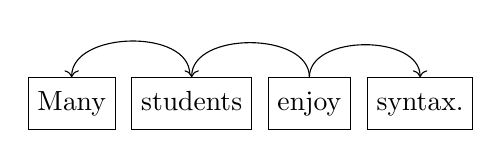
\begin{tikzpicture}[node distance=.2cm]
\node[draw](many) at (0,0){\strut{Many}};
\node[draw](students) [right=of many]{\strut students};
\node[draw](enjoy) [right=of students]{\strut enjoy};
\node[draw](syntax) [right= of enjoy]{\strut syntax.};
\draw[->] (enjoy)[out=north,in=north] to (syntax);
\draw[->] (enjoy)[out=north,in=north] to (students);
\draw[->] (1.5,.37)[out=north,in=north] to (many);
\end{tikzpicture}
%
	\caption{Phrase structure and dependency structure contrasted}
	\label{fig:1}
\end{figure}

In both approaches, each unit has properties such as a classification, a meaning, a form and relations to other items, but these properties may be thought of in two different ways. In PS analyses, an item contains its related items so it also contains its other properties – hence the familiar AVMs contained within the box for each item. But in DS analyses, an item’s related items are outside it, sitting alongside it in the analysis, so for consistency other properties may be shown as a network in which the item concerned is just one atomic node. This isn’t the only possible notation, but it is the basis for the main DS theory that I shall juxtapose with HPSG, Word Grammar.

What, then, are the distinctive characteristics of the two traditions? In the following summary I use \emph{item} to include any syntagmatic unit of analysis including morphemes, words and phrases (though this chapter will not discuss the possible role of morphemes). The following generalisations apply to classic examples of the two approaches: PS as defined by Chomsky in terms of labelled bracketed strings \citep{Chomsky57a}, and DS as defined by \citeauthor{Tesniere59a-u} (\citeyear{Tesniere59a-u,Tesniere2015a-u}). These generalisations refer to “direct relations”, which are shown by single lines in standard tree notation; for example, taking a pair of words such as \emph{big book}, they are related directly in DS, but only indirectly via a mother phrase in PS. A phenomenon such as agreement is not a relation in this sense, but it applies to word-pairs which are identified by their relationship; so even if two sisters agree, this does not in itself constitute a direct relation between them.

\begin{enumerate}
	\item\label{it:1} Containment: in PS, but not in DS, if two items are directly related, one must contain the other. For instance, a PS analysis of \emph{the book} recognises a direct relation (of dominance) between book and \emph{the book}, but not between \emph{book} and \emph{the}, which are directly related only by linear precedence. In contrast, a DS analysis does recognise a direct relation between \emph{book} and \emph{the} (in addition to the linear precedence relation).
	
	\item\label{it:2}  Continuity: therefore, in PS, but not in DS, all the items contained in a larger one must be adjacent.
	
	\item\label{it:3} Asymmetry: in both DS and PS, a direct relation between two items must be asymmetrical, but in DS the relation (between two words) is dependency whereas in PS it is the part-whole relation.
\end{enumerate}

These generalisations imply important theoretical claims which can be tested; for instance, \ref{it:2} claims that there are no discontinuous phrases, which is clearly false. On the other hand, \ref{it:3} claims that there can be no exocentric or headless phrases, so DS has to consider apparent counter-examples such as NPN constructions, coordination and verbless sentences (see Sections \ref{sec:4.2} and \ref{sec:5.1} for discussion, and also the chapter on coordination).

The contrasts in \ref{it:1}--\ref{it:3} apply without reservation to ‘plain vanilla’ \citep{Zwicky85a} versions of DS and PS, but as we shall see in the history section, very few theories are plain vanilla. In particular, there are versions of HPSG that allow phrases to be discontinuous \citep{Reape94a,Kathol2000a,Mueller95c,Babel}. Nevertheless, the fact is that HPSG evolved out of more or less pure PS, that it includes \emph{phrase structure} in its name, and that it is never presented as a version of DS.

On the other hand, the term \emph{Head-driven} points immediately to dependency: an asymmetrical relation driven by a head word. Even if HPSG gives some constructions a headless analysis \citep[654-666]{MuellerGT-Eng2}, the fact remains that it treats most constructions as headed.
This chapter reviews the relations between HPSG and the very long DS tradition of grammatical analysis. The conclusion will be that in spite of its PS roots, HPSG implicitly (and sometimes even explicitly) recognises dependencies; and it may not be a coincidence that one of the main power-bases of HPSG is Germany, where the DS tradition is also at its strongest  \citep[359]{MuellerGT-Eng2}.

Where, then, does this discussion leave the notion of a phrase? In PS, phrases are basic units of the analysis, alongside words; but even DS recognises phrases indirectly because they are easily defined in terms of dependencies as a word plus all the words which depend, directly or indirectly, on it. Although phrases play no part in a DS analysis, it is sometimes useful to be able to refer to them informally (in much the same way that some PS grammars refer to grammatical functions informally while denying them any formal status).

Why, then, does HPSG use PS rather than DS? As far as I know, PS was simply default syntax in the circles where HPSG evolved, so the choice of PS isn’t the result of a conscious decision by the founders, and I hope that this chapter will show that this is a serious question which deserves discussion%
%
\footnote{Indeed, I once wrote a paper (which was never published) called Taking the PS out of HPSG – a title I was proud of until I noticed that PS was open to misreading, not least as “Pollard and Sag”. Carl and Ivan took it well, and I think Carl may even have entertained the possibility that I might be right – possibly because he had previously espoused a theory called “Head Grammar” (HG).}%
%
. Unfortunately, the historical roots and the general dominance of PS have so far discouraged discussion of this fundamental question.

HPSG is a theoretical package where PS is linked intimately to a collection of other assumptions; and the same is true for any theory which includes DS, including my own Word Grammar
\cite{Hudson84a-u,Hudson90a-u,Hudson98a-u,Hudson2007a-u,Hudson2010b-u}%
%
\todo{Gisborne 2010; Duran-Eppler 2011; Traugott\&Trousdale 2013}%
\todo{forthcoming???}%
%
. Among the other assumptions of HPSG I find welcome similarities, not least the use of default inheritance in some versions of the theory. I shall argue below that inheritance offers a novel solution to one of the outstanding challenges for the dependency tradition.

The next section sets the historical scene. This is important because it’s all too easy for students to get the impression (mentioned above) that PS is just default syntax, and maybe even the same as “traditional grammar”. We shall see that grammar has a very long and rather complicated history in which the default is actually DS rather than PS. Later sections then address particular issues shared by HPSG and the dependency tradition.


%%%%%%%%%%%%%%%%%%%%%%%%%%%%%%%%%%%%%%%%%%%%%%%%%%%%%
%%%%%%%%%%%%%%%%%%%%%%%%%%%%%%%%%%%%%%%%%%%%%%%%%%%%%
\section{Dependency and constituency in the history of syntax}
\label{sec:2}

The relevant history of syntax starts more than two thousand years ago in Greece. (Indian syntax may have started even earlier, but it is hardly relevant because it had so little impact on the European tradition.) Greek and Roman grammarians focused on the morphosyntactic properties of individual words, but since these languages included a rich case system, they were aware of the syntactic effects of verbs and prepositions governing particular cases. However, this didn’t lead them to think about syntactic relations, as such; precisely because of the case distinctions, they could easily distinguish a verb’s dependents in terms of their cases: “its nominative”, “its accusative” and so on \todo{Robins 1967, 29}. Both the selecting verb or preposition and the item carrying the case inflection were single words, so the Latin grammar of Priscian, written about 500 AD and still in use a thousand years later, recognised no units larger than the word: “his model of syntax was word-based – a dependency model rather than a constituency model” \todo{Law 2003, 91}. However, it was a dependency model without the notion of dependency as a relation between words.

The dependency relation, as such, seems to have been first identified by the Arabic grammarian Sibawayh in the 8\textsuperscript{th} century \todo{Owens 1988; Kouloughli 1999}. However, it is hard to rule out the possibility of influence from the then-flourishing Paninian tradition in India, and in any case it doesn’t seem to have had any more influence on the European tradition than did Panini’s syntax, so it is probably irrelevant.

In Europe, grammar teaching in schools was based on parsing (in its original sense), an activity which was formalised in the ninth century \todo{Luhtala 1994}. The activity of parsing was a sophisticated test of grammatical understanding which earned the central place in school work that it held for centuries – in fact, right up to the 1950s (when I myself did parsing at school) and maybe beyond. In HPSG terms, school children learned a standard list of attributes for words of different classes, and in parsing a particular word in a sentence their task was to provide the values for its attributes, including its grammatical function (which would explain its case). In the early centuries the language was Latin, but more recently it was the vernacular (in my case, English).

Alongside these purely grammatical analyses, the Ancient World had also recognised a logical one, due to Aristotle, in which the basic elements of a proposition (\emph{logos}) are the logical subject (\emph{onoma}) and the predicate (\emph{rhēma}). For Aristotle a statement such as “Socrates ran” requires the recognition both of the person Socrates and of the property of running, neither of which could constitute a statement on its own \todo{(Law 2003, 30–31)}. By the twelfth century, grammarians started to apply a similar analysis to sentences; but in recognition of the difference between logic and grammar they replaced the logicians’ \emph{subiectum} and \emph{praedicatum} by \emph{suppositum} and \emph{appositum} – though the logical terms would creep into grammar by the late eighteenth century \todo{(Law 2003, 168)}. This logical analysis produced the first top-down analysis in which a larger unit (the logician’s proposition or the grammarian’s sentence) has parts, but the parts were still single words, so \emph{onoma} and \emph{rhēma} can now be translated as ‘noun’ and ‘verb’. If the noun or verb was accompanied by other words, the older dependency analysis applied.

The result of this confusion of grammar with logic was a muddled hybrid analysis in the Latin/Greek tradition which combines a headless subject-predicate analysis with a headed analysis elsewhere, and which persists even today in some school grammars; this confusion took centuries to sort out in grammatical theory. For the subject and verb, the prestige of Aristotle and logic supported a subject-verb division of the sentence (or clause) in which the subject noun and the verb were both equally essential – a very different analysis from modern first-order logic in which the subject is just one argument (among many) which depends on the predicate. Moreover the grammatical tradition even includes a surprising number of analyses in which the subject noun is the head of the construction, ranging from the modistic grammarians of the twelfth century\todo{Robins 1967, 83}, through Henry Sweet\todo{Sweet 1891, 17}, to no less a figure than Otto Jespersen in the twentieth \citep{Jespersen37a-u}, who distinguished ‘junction’ (dependency) from ‘nexus’ (predication) and treated the noun in both constructions as ‘primary’.

The first grammarians to recognise a consistently dependency-based analysis for the rest of the sentence (but not for the subject and verb) seem to have been the French \emph{encyclopédistes} of the eighteenth century \todo{(Kahane forthcoming)}, and by the nineteenth century much of Europe accepted a theory of sentence structure based on dependencies, but with the subject-predicate analysis as an exception – an analysis which by modern standards is muddled and complicated. Each of these units was a single word, not a phrase, and modern phrases were recognised only indirectly by allowing the subject and predicate to be expanded by dependents; so nobody ever suggested there might be such a thing as a noun phrase until the late nineteenth century. Function words such as prepositions had no proper position, being treated typically as though they were case inflections.

The invention of syntactic diagrams in the nineteenth century made the inconsistency of the hybrid analysis obvious. The first such diagram was published in a German grammar of Latin for school children \todo{(Billroth 1832)}, and the nineteenth century saw a proliferation of diagramming systems%
%
\footnote{See a small selection at \url{http://dickhudson.com/sentence-diagramming/}. (Last access October 2018.)}%
%
, including the famous Reed-Kellogg diagrams which are still taught (under the simple name ‘diagramming’) in some American schools \citep{RK1877a}; indeed, there is a website%
%
\footnote{Sentence Diagrammer by 1aiway at \url{https://download.cnet.com/windows/1aiway/3260-20_4-10725918-1.html}. (Last access January 2019)}%
%
 which generates such diagrams, giving diagrams such as the one reproduced in Figure \ref{fig:2}. The significant feature of this diagram is the special treatment given to the relation between the subject and predicate (with the verb \emph{are} sitting uncomfortably between the two), with all the other words in the sentence linked by more or less straightforward dependencies. (The geometry of these diagrams also distinguishes grammatical functions.)
 
 \begin{figure}
 	\centering
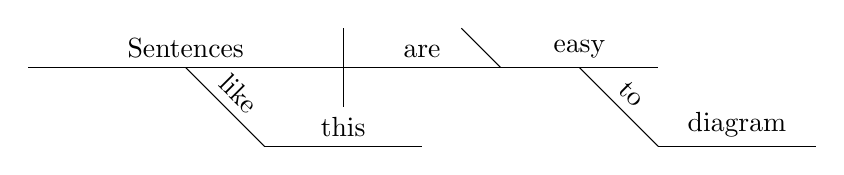
\begin{tikzpicture}
\draw (0,0) to [edge label=Sentences] (4,0);
\draw (4,.5) to (4,-.5);
\draw (2,0) to [edge label=like,sloped] (3,-1);
\draw (3,-1) to [edge label=this] (5,-1);
\draw (4,0) to [edge label=are] (6,0);
\draw (6,0) to (5.5,.5);
\draw (6,0) to [edge label=easy,sloped] (8,0);
\draw (7,0) to [edge label=to,sloped] (8,-1);
\draw (8,-1) to [edge label=diagram] (10,-1);
\end{tikzpicture}
	\caption{Reed and Kellogg diagram by Sentence Diagrammer}
	\label{fig:2}
 \end{figure}
 
One particularly interesting (and relevant) fact about Reed and Kellogg is that they offer an analysis of that old wooden house in which each modifier creates a new unit to which the next modifier applies: \emph{wooden house}, then \emph{old wooden house} \todo{Percival 1976, 18} – a clear hint at more modern structures (including the ones proposed in Section \ref{sec:4.1}, albeit one that sits uncomfortably with plain-vanilla dependency structure.
 
However, even in the nineteenth century there were grammarians who questioned the hybrid tradition which combined the subject-predicate distinction with dependencies. Rather remarkably, three different grammarians seem to have independently reached the same conclusion at roughly the same time: hybrid structures can be replaced by a homogeneous structure if we take the finite verb as the root of the whole sentence, with the subject as one of its dependents. This idea seems to have been first proposed in print in 1873 by the Hungarian Sámuel Brassai \citep{Imrenyi2013a} \todo{Imrényi and Vladár forthcoming}; in 1877 by the Russian Aleksej Dmitrievsky \todo{Sériot 2004}; and in 1884 by the German Franz Kern \citep{Kern1884a-u}. Both Brassai and Kern used diagrams to present their analyses, and used precisely the same tree-structures which Lucien Tesnière in France called “stemmas” nearly fifty years later \citep{Tesniere59a-u,Tesniere2015a-u}. The diagrams have both been redrawn here as Figures \ref{fig:3} and \ref{fig:4}.

\begin{figure}
	\centering
\begin{forest}
[\emph{tenebat}\\governing verb
	[\emph{flentem}\\dependent]
	[\emph{Uxor}\\dependent
		[\emph{amans}\\attribute]
		[\emph{ipsa}\\attribute]
		[\emph{flens}\\attribute
			[\emph{acrius}\\tertiary\\dependent]
		]
	]
	[\emph{imbre cadente}\\dependent
		[\emph{usque}\\secondary\\dependent]
		[\emph{per genas}\\secondary\\dependent
			[\emph{indignas}\\tertiary\\dependent]
		]
	]
]
\end{forest}
	\caption{A verb-rooted tree from Brassai 1873}
	\label{fig:3}
\end{figure}\todo{Brassai 1873}	

 
Brassai’s proposal is contained in a school grammar of Latin, so the example is also from Latin – an extraordinarily complex sentence which certainly merits a diagram.

\begin{exe}
	\ex \label{ex:1}
	\gll Uxor am -ans fl -ent -em fl -ens acr -ius ips -a ten -eb -at, imbr -e per in -dign -as usque cad -ent -e gen -as.\\
	wife\textsc{.f.sg.nom} love \textsc{-ptcp.f.sg.nom} cry \textsc{-ptcp} \textsc{-m.sg.acc} cry \textsc{-ptcp.f.sg.nom} bitterly -more self \textsc{-f.sg.nom} hug \textsc{-pst} \textsc{-3.sg} shower \textsc{-m.sg.abl} on un -becoming \textsc{-f.pl.acc} continuously fall \textsc{-ptcp} \textsc{-m.sg.abl} cheeks \textsc{-f.pl.acc}\\
	\glt ‘The wife, herself even more bitterly crying, was hugging the crying one, while a shower [of tears] was falling on her unbecoming cheeks [i.e. cheeks to which tears are unbecoming].’
\end{exe}

Brassai’s diagram, including grammatical functions as translated by the authors \todo{(Imrényi and Vladár forthcoming???)}, is in Figure \ref{fig:3}. The awkward horizontal braces should not be seen as a nod in the direction of classical PS given that the bracketed words are not even adjacent in the sentence analysed. Kern’s tree in Figure \ref{fig:4}, on the other hand, is for the German sentence in (\ref{ex:2}).

\begin{exe}
	\ex \label{ex:2}
	\gll Ein -e stolz -e Krähe schmück -t -e sich mit d -en aus {-gefall -en -en} Feder -n d -er {Pfau -en}.\\
	a \textsc{-f.sg.nom} proud \textsc{-f.sg.nom} crow\textsc{.f.sg.nom} decorate \textsc{-pst} \textsc{-3.sg} self\textsc{.acc} with the \textsc{-f.pl.dat} out -fall\textsc{.ptcp.f.pl.dat} feather \textsc{-f.pl.dat} the \textsc{-m.pl.gen} peacock\textsc{.m.pl.gen}\\
	\glt ‘A proud crow decorated himself with the dropped feathers of the peacocks.’
\end{exe}

Once again, the original diagram includes function terms which are translated in this diagram into English.

\begin{figure}
	\centering
\begin{forest}
[\emph{schmückte}\\finite verb
	[\emph{Krähe}\\subject word
		[\emph{eine}\\counter]
		[\emph{stolze}\\attributive adjective]
	]
	[\emph{sich}\\object]
	[\emph{mit Federn}\\case with preposition
		[\emph{den}\\pointer]
		[\emph{ausgefallenen}\\attributive adjective\\(participle)]
		[\emph{Pfauen}\\genitive
			[\emph{der}\\pointer]
		]
	]
]
\end{forest}
	\caption{A verb-rooted tree from \citealp{Kern1884a-u}}
	\label{fig:4}
\end{figure}


Once again the analysis gives up on prepositions, treating mit Federn (‘with feathers’) as a single word, but Figure \ref{fig:4} is an impressive attempt at a coherent analysis which would have provided an excellent foundation for the explosion of syntax in the next century. According to the classic history of dependency grammar, in this approach,

\begin{quotation}
	[\dots] the sentence is not a basic grammatical unit, but merely results from combinations of words, and therefore [\dots] the only truly basic grammatical unit is the word. A language, viewed from this perspective, is a collection of words and ways of using them in word-groups, i.e., expressions of varying length. \todo{Percival 1976, 21}
\end{quotation}

But the vagaries of intellectual history and geography worked against this intellectual breakthrough. When Leonard Bloomfield was looking for a theoretical basis for syntax, he could have built on what he had learned at school:

\begin{quotation}
	[\dots] we do not know and may never know what system of grammatical analysis Bloomfield was exposed to as a schoolboy, but it is clear that some of the basic conceptual and terminological ingredients of the system that he was to present in his 1914 and 1933 books were already in use in school grammars of English current in the United States in the nineteenth century. Above all, the notion of sentence “analysis”, whether diagramable or not, had been applied in those grammars. \todo{Percival 1976, 18}
\end{quotation}

And when he visited Germany in 1913--14 he might have learned about Kern’s ideas which were already influential there. But instead, he adopted the syntax of the German psychologist Wilhelm Wundt. Wundt’s theory applied to meaning rather than syntax, and was based on a single idea: that every idea consists of a subject and a predicate. For example, a phrase meaning “a sincerely thinking person” has two parts: \emph{a person} and thinks sincerely; and the latter breaks down, regardless of the grammar, into the noun \emph{thought} and \emph{is sincere} \todo{Percival 1976}.

For all its reliance on logic rather than grammar, the analysis is a clear precursor to neo-Bloomfieldian trees: it recognises a single consistent part-whole relationship (a partonomy) which applies recursively. This, then, is the beginning of the PS tradition: an analysis based purely on meaning as filtered through a speculative theory of cognition – an unpromising start for a theory of syntax. However, Bloomfield’s school experience presumably explains why he combined Wundt’s partonomies with the hybrid structures of Reed-Kellogg diagrams in his classification of structures as endocentric (headed) or exocentric (headless). For him, exocentric constructions include the subject-predicate structure and preposition phrases, both of which were problematic in sentence analysis at school. Consequently, his Immediate Constituent Analysis (ICA) perpetuated the old hybrid mixture of headed and headless structures.

The DS elements of ICA are important in evaluating the history of PS, because they contradict the standard view of history expressed here:

\begin{quotation}
	Within the Bloomfieldian tradition, there was a fair degree of consensus regarding the application of syntactic methods as well as about the analyses associated with different classes of constructions. Some of the general features of IC analyses find an obvious reflex in subsequent models of analysis. Foremost among these is the idea that structure involves a part–whole relation between elements and a larger superordinate unit, rather than an asymmetrical dependency relation between elements at the same level. \todo{Blevins and Sag 2013, 202–3}
\end{quotation}

This quotation implies, wrongly, that ICA rejected DS altogether.

What is most noticeable about the story so far is that even in the 1950s we still haven’t seen an example of pure phrase structure. Every theory visited so far has recognised dependency relations in at least some constructions. Even Bloomfieldian ICA had a place for dependencies, though it introduced the idea that dependents might be phrases rather than single words and it rejected the traditional grammatical functions such as subject and object. Reacting against the latter gap, and presumably remembering their schoolroom training, some linguists developed syntactic theories which were based on constituent structure but which did have a place for grammatical functions, though not for dependency as such. The most famous of these theories are Tagmemics \todo{Pike 1954} and Systemic Functional Grammar \todo{Halliday 1961;} \citep{Halliday67b-u}. However, in spite of its very doubtful parentage and its very brief history, by the 1950s virtually every linguist in America seemed to accept without question the idea that syntactic structure was a partonomy.

This is the world in which Noam Chomsky introduced phrase structure, which he presented as a formalisation of ICA, arguing that “customarily, linguistic description on the syntactic level is formulated in terms of constituent analysis (parsing)” \citep[26]{Chomsky57a}. But such analysis was only “customary” among the Bloomfieldians, and was certainly not part of the classroom activity of parsing \todo{Matthews 1993, 147}.

Chomsky’s phrase structure continued the drive towards homogeneity which had led to most of the developments in syntactic theory since the early nineteenth century. Unfortunately, Chomsky dismissed both dependencies and grammatical functions as irrelevant clutter, leaving nothing but part-whole relations, continuity and sequential order, and category-labels.

Rather remarkably, the theory of phrase structure implied the (psychologically implausible) claim that sideways relations such as dependencies between individual words are impossible in a syntactic tree – or at least that, even if they are psychologically possible, they can (and should) be ignored in a formal model. Less surprisingly, having defined PS in this way, he could easily prove that it was inadequate and needed to be greatly expanded beyond the plain-vanilla version. His solution was the introduction of transformations, but it was only thirteen years before he also recognised the need for some recognition of head-dependent asymmetries in X-bar theory \citep{Chomsky70a}. At the same time, others had objected to transformations and started to develop other ways of making PS adequate. One idea was to include grammatical functions; this idea was developed variously in LFG \citep{Bresnan78a,Bresnan2001a}, Relational Grammar \citep{PP83b-u} \todo{Blake 1990} and Functional Grammar \todo{Dik 1989; Siewierska 1991}. Another way forward was to greatly enrich the categories \citep{Harman63a} as in GPSG \citep{GKPS85a} and HPSG \citep{ps2}. 

Meanwhile, the European ideas about syntactic structure culminating in Kern’s tree diagram developed rather more slowly. Lucien Tesnière in France wrote the first full theoretical discussion of DS in 1939 but it was not published till 1959 \citep{Tesniere59a-u,Tesniere2015a-u}, complete with stemmas looking like the diagrams produced seventy years earlier by Brassai and Kern. Somewhat later, these ideas were built into theoretical packages in which DS was bundled with various other assumptions about levels and abstractness. Here the leading players were from Eastern Europe, where DS flourished: the Russian Igor Mel’čuk \citep{Melcuk88a-u}, who combined DS with multiple analytical levels, and the Czech linguists Petr Sgall, Eva Hajičová and Jarmila Panevova \todo{Sgall, Hajicová, and Panevova 1986}, who included information structure. My own theory Word Grammar (developed, exceptionally, in the UK), also stems from the 1980s \citep{Hudson84a-u,Hudson90a-u,Hudson2007a-u,Hudson2010b-u,Hudson2017a} \todo{Sugayama 2002; Gisborne 2008; Rosta 2008; Gisborne 2010; Gisborne 2011; Duran-Eppler 2011; Traugott and Trousdale 2013; Duran Eppler, Luescher, and Deuchar 2016; Hudson 2016; 2017; Gisborne 2019}. This is the theory which I compare below with HPSG, but it is important to remember that other DS theories would give very different answers to some of the questions that I raise.

DS certainly has a low profile in theoretical linguistics, and especially so in anglophone countries, but there is an area of linguistics where its profile is much higher (and which is of particular interest to the HPSG community): natural-language processing \citep{KMcDN2009a-u}. For example:

\begin{itemize}
	\item the Wikipedia entry for “Treebank” classifies 50 of its 101 treebanks as using dependency structure%
	%
	\footnote{\url{https://en.wikipedia.org/wiki/Treebank} (January 2019)}%
	%
	.
	
	\item The “Universal dependencies” website lists more than 100 dependency-based treebanks for 60 languages%
	%
	\footnote{\url{https://universaldependencies.org/} (January 2019)}%
	%
	.
	
	\item Google’s n-gram facility allows searches based on dependencies%
	%
	\footnote{\url{https://books.google.com/ngrams/info} and search for ‘dependency’. (January 2019)}%
	%
	.
	
	\item The Stanford Parser (Chen and Manning 2014; de Marneffe et al. 2014) uses DS%
	%
	\footnote{\url{https://nlp.stanford.edu/software/stanford-dependencies.shtml} (January 2019)}%
	%
	.
\end{itemize}

The attraction of DS in NLP is that the only units of analysis are words, so at least these units are given in the raw data and the overall analysis can immediately be broken down into a much simpler analysis for each word. This is as true for a linguist building a treebank as it was for a school teacher teaching children to parse words in a grammar lesson. Of course, as we all know, the analysis actually demands a global view of the entire sentence, but at least in simple examples a bottom-up word-based view will also give the right result.

To summarise this historical survey, PS is a recent arrival, and is not yet a hundred years old. Previous syntacticians had never considered the possibility of basing syntactic analysis on a partonomy. Instead, it had seemed obvious that syntax was literally about how words (not phrases) combined with one another.


%%%%%%%%%%%%%%%%%%%%%%%%%%%%%%%%%%%%%%%%%%%%%%%%%%%%%
%%%%%%%%%%%%%%%%%%%%%%%%%%%%%%%%%%%%%%%%%%%%%%%%%%%%%
\section{HPSG and Word Grammar}
\label{sec:3}

The rest of this chapter considers a number of crucial issues that distinguish PS and DS by focusing specifically on how they distinguish two particular manifestations of these traditions, HPSG and Word Grammar (WG). The main question is, of course, how strong the evidence is for the PS basis of HPSG, and how easily this basis could be replaced by DS.

The comparison requires some understanding of WG, so what follows is a brief tutorial on the parts of the theory which will be relevant in the following discussion. Like HPSG, WG combines claims about syntactic relations with a number of other assumptions; but for WG, the main assumption is the Cognitive Principle:

\begin{description}
	\item[The Cognitive Principle] \label{it:CogPrin}Language uses the same general cognitive processes and resources as general cognition, and has access to all of them.
\end{description}

This principle is of course merely a hypothesis which may turn out to be wrong, but so far it seems correct \citep[494]{MuellerGT-Eng2}, and it is more compatible with HPSG than with the innatist ideas underlying Chomskyan linguistics \todo{Berwick et al. 2013}. In WG, it plays an important part because it determines other parts of the theory.

On the one hand, cognitive psychologists tend to see knowledge as a network of related concepts \todo{Reisberg 2007, 252}, so WG also assumes that the whole of language, including grammar, is a conceptual network (\citealt[1]{Hudson84a-u}; \citeyear[1]{Hudson2007a-u}). One of the consequences is that the AVMs of HPSG are presented instead as labelled network links; for example, we can compare the elementary example in Figure \ref{fig:5} of the HPSG lexical item for a German noun \citep[264]{MuellerGT-Eng2} with an exact translation using WG notation.

\begin{figure}
	\centering
\onems[word]{
	phonology    \phonliste{ Grammatik } \\[1mm]
	syntax-semantics  \ldots \ms[local]{ category  & \ms[category]{ head & \ms[noun]{ case & \ibox{1}
			}\\[3mm]
			spr & \sliste{ Det[\textsc{case}~\ibox{1}] }\\
			\ldots\\
		} \\[10mm]
		content & \ldots \ms[grammatik]{ inst & X 
		}
	}
}
%\vspace{-\baselineskip}
	\caption{An AVM for the German noun \emph{Grammatik}}
	\label{fig:5}
\end{figure}

HPSG regards AVMs as equivalent to networks, so translating this AVM into network notation is straightforward; however it is visually complicated so I take it in two steps. First I introduce the basic notation in Figure \ref{fig:6}: a small triangle showing that the lexeme \textsc{grammatik} “isa” word, and a headed arrow representing a labelled attribute (here, “phonology”) and pointing to its value. The names of entities and attributes are enclosed in rectangles and ellipses respectively.

\begin{figure}
	\centering
\begin{tikzpicture}[node distance=3cm]
\node[draw](word) at (0,1.5){word};
\node[draw](grammatik) at (0,0){\textsc{grammatik}};
\node[draw,ellipse](phonology) [right of=grammatik]{phonology};
\node[draw](Grammatik) [right of=phonology]{\emph{Grammatik}};
\draw[<-,>=open triangle 90 reversed] (word) to (grammatik);
\draw (phonology) to (grammatik);
\draw[->] (phonology) to (Grammatik);
\end{tikzpicture}
	\caption{The German noun \emph{Grammatik}, ‘grammar’, in a WG network}
	\label{fig:6}
\end{figure}

The rest of the AVM translates quite smoothly (ignoring the list for \textsc{spr}), giving Figure \ref{fig:7}, though an actual WG analysis would be rather different in ways that are irrelevant here.

\begin{figure}
	\centering
\begin{tikzpicture}[node distance=1.8cm]
%relative placement of nodes starting from 1
\node[draw](1) at (0,0){1};
\node[draw,ellipse](case1)[above left of=1]{case};
\node[draw,ellipse](case2)[above right of=1]{case};
\node[draw](noun)[above left of=case1]{\emph{noun}};
\node[draw](det)[above right of=case2]{\emph{det}};
\node[draw,ellipse](head)[above right of=noun]{head};
\node[draw,ellipse](spr)[above left of=det]{spr};
\node[draw](category1)[above left of=spr]{\emph{category}};
\node[draw,ellipse](category2)[above right of=category1]{category};
\node[draw](local)[above right of=category2]{\emph{local}};
\node[draw,ellipse](content)[below right of=local]{content};
\node[draw](grammatik1)[below right of=content]{\emph{grammatik}};
\node[draw,ellipse](inst)[below of=grammatik1]{inst};
\node[draw](X)[below of=inst]{X};
\node[draw,ellipse](synsem)[above of=local]{syntax-semantics};
\node[draw](grammatik2)[above of=synsem]{\textsc{grammatik}};
%arrows (I didnt manage to find a way to whitefill the ellipses afterwards, so every arrow is split up :/)
\draw (grammatik2) to (synsem);
\draw[->] (synsem) to (local);
\draw (local) to (category2);
\draw (local) to (content);
\draw[->] (category2) to (category1);
\draw[->] (content) to (grammatik1);
\draw (grammatik1) to (inst);
\draw[->] (inst) to (X);
\draw (category1) to (head);
\draw (category1) to (spr);
\draw[->] (head) to (noun);
\draw[->] (spr) to (det);
\draw (noun) to (case1);
\draw (det) to (case2);
\draw[->] (case1) to (1);
\draw[->] (case2) to (1);
\end{tikzpicture}
	\caption{The German noun \emph{Grammatik}, ‘grammar’, in a WG network}
	\label{fig:7}
\end{figure}

The other difference based on cognitive psychology between HPSG and WG is that many cognitive psychologists argue that concepts are built around prototypes \todo{Rosch 1973; Taylor 1995}, clear cases with a periphery of exceptional cases. This claim implies the logic of default inheritance \citep{BCdP93a-ed}, which is popular in AI though less so in logic. In HPSG, default inheritance is accepted by some \citep{LC99a} but not by others \citep[403]{MuellerGT-Eng2}, whereas in WG it plays a fundamental role, as I show in Section \ref{sec:4.1} below. WG uses the ‘isa’ relation to carry default inheritance, and avoids the problems of non-monotonic inheritance by restricting inheritance to node-creation \cite[18]{Hudson2017a}. Once again, the difference is highly relevant to the comparison of PS and DS because one of the basic questions is whether syntactic structures involve partonomies (based on whole:part relations) or taxonomies (based on the isa relation). (I argue in Section \ref{sec:4.1} that taxonomies exist within the structure of a sentence thanks to isa relations between tokens and sub-tokens.)

Default inheritance leads to an interesting comparison of the ways in which the two theories treat attributes. On the one hand, they both recognise a taxonomy in which some attributes are grouped together as similar; for example, the HPSG analysis in Figure 5 classifies the attributes \textsc{category} and \textsc{content} as \textsc{local}, and within \textsc{category} it distinguishes the \textsc{head} and \textsc{specifier} attributes. In WG attributes are called relations, and they too form a taxonomy. The simplest examples to present are the traditional grammatical functions, which are all subtypes of “dependent”; for example, “object” isa “complement”, which isa “valent”, which isa “dependent”, as shown in Figure \ref{fig:8} (which begs a number of analytical questions such as the status of depictive predicatives, which are not complements).

\begin{figure}
	\centering
\begin{tikzpicture}[>=open triangle 90 reversed]
\node[shape=ellipse,draw](object) at (0,0) {object};
\node[shape=ellipse,draw](complement) at (0,1.5) {complement};
\node[shape=ellipse,draw](valent) at (0,3) {\strut{valent}};
\node[shape=ellipse,draw](dependent) at (0,4.5) {dependent};
\node[shape=ellipse,draw](predicative) at (3,0) {predicative};
\node[shape=ellipse,draw](adjunct) at (3,1.5) {adjunct};
\node[shape=ellipse,draw](subject) at (3,3) {subject};
\draw[<-] (dependent) to (valent);
\draw (subject) to (0,3.925);
\draw[<-] (valent) to (complement);
\draw (adjunct) to (0,2.34);
\draw[<-] (complement) to (object);
\draw (predicative) to (0,0.925);
\end{tikzpicture}
	\caption{A WG taxonomy of grammatical functions}
	\label{fig:8}
\end{figure}

In spite of the differences in the categories recognised, the formal similarity is striking. On the other hand, there is also an important formal difference in the roles played by these taxonomies. In spite of interesting work on default inheritance \citep{LC99a}, most versions of HPSG allow generalisations but not exceptions (“If one formulates a restriction on a supertype, this automatically affects all of its subtypes.” \citep[275]{MuellerGT-Eng2}), whereas in WG the usual logic of default inheritance applies so exceptions are possible. These are easy to illustrate from word order, which (as explained in Section \ref{sec:4.4}) is normally inherited from dependencies: a verb’s subject normally precedes it, but an inverted subject (the subject of an inverted auxiliary verb, as in \emph{did he}) follows it.

Another reason for discussing default inheritance and the isa relation is to explain that WG, just like HPSG, is a constraint-based theory. In HPSG, a sentence is grammatical if it can be modeled given the structures and lexicon provided by the grammar, which are combined with each other via unification. Similarly, in WG it is grammatical if its word tokens can all be inherited from entries in the grammar (which, unlike HPSG, also includes the entire lexicon). Within the grammar, these may involve overrides but overrides between the grammar and the word tokens imply some degree of ungrammaticality. For instance, \emph{He slept} is grammatical because all the properties of \emph{He} and \emph{slept} (including their syntactic properties such as the word order that can be inherited from their grammatical function) can be inherited directly from the grammar, whereas *\emph{Slept he} is ungrammatical in that the order of words is exceptional, and the exception is not licensed by the grammar.

This completes the tutorial on WG, so we are now ready to consider the issues that distinguish HPSG from this particular version of DS. In preparation for this discussion, I return to the three distinguishing assumptions about classical PS and DS theories given earlier as \ref{it:1} to \ref{it:3}, and repeated here:

\begin{enumerate}
	\item Containment: in PS, but not in DS, if two items are directly related, one must contain the other.
	
	\item Continuity: therefore, in PS, but not in DS, all the items contained in a larger one must be adjacent.
	
	\item Asymmetry: in both DS and PS, a direct relation between two items must be asymmetrical, but in DS the relation (between two words) is dependency whereas in PS it is the part-whole relation.
\end{enumerate}

These distinctions will provide the structure for the discussion:

\begin{itemize}
	\item  Containment and continuity:
	\begin{itemize}
		\item Semantic phrasing
		
		\item Coordination
		
		\item Phrasal edges
		
		\item Word order
	\end{itemize}

	\item Asymmetry:
	\begin{itemize}
		\item Structure sharing and raising/lowering
		
		\item Headless phrases
		
		\item Complex dependency
		
		\item Grammatical functions
	\end{itemize}
\end{itemize}


%%%%%%%%%%%%%%%%%%%%%%%%%%%%%%%%%%%%%%%%%%%%%%%%%%%%%
%%%%%%%%%%%%%%%%%%%%%%%%%%%%%%%%%%%%%%%%%%%%%%%%%%%%%
\section{Containment and continuity (PS but not DS)}
\label{sec:4}

%%%%%%%%%%%%%%%%%%%%%%%%%%%%%%%%
\subsection{Semantic phrasing}
\label{sec:4.1}

One apparent benefit of PS is what I call “semantic phrasing” \citep[146-151]{Hudson90a-u}, in which the effect of adding a dependent to a word modifies that word’s meaning to produce a different meaning. For instance, the phrase \emph{typical French house} does not mean ‘house which is both typical and French’, but rather ‘French house which is typical (of French houses)’ \citep{Dahl80a}. In other words, even if the syntax does not need a node corresponding to the combination \emph{French house}, the semantics does need one.

For HPSG, of course, this is not a problem because every dependent is part of a new structure, semantic as well as syntactic \citep{MuellerEvaluating}; so the syntactic phrase \emph{French house} has a content which is ‘French house’. But for DS theories, this is not generally possible because there is no syntactic node other than those for individual words – so, in this example, one node for \emph{house} and one for \emph{French} but none for \emph{French house}.

Fortunately for DS, there is a solution: create extra word nodes but treat them as a taxonomy, not a partonomy \todo{Hudson 2018}. To appreciate the significance of this distinction, the connection between the concepts “finger” and “hand” is a partonomy, but that between “index finger” and “finger” is a taxonomy; a finger is part of a hand, but it is not a hand, and conversely an index finger is a finger, but it is not part of a finger.

In this analysis, then, the token of \emph{house} in \emph{typical French house} would be factored into three distinct nodes:

\begin{description}
	\item[\emph{house}:] \label{it:house} an example of the lexeme \textsc{house}, with the inherited meaning ‘house’.
	
	\item [\emph{house+F}:] \label{it:house+f} the word \emph{house} with \emph{French} as its dependent, meaning ‘French house’.
	
	\item[\emph{house+t}:] \label{it:house+t} the word \emph{house+F} with \emph{typical} as its dependent, meaning ‘typical example of a French house’.
\end{description}

(It is important to remember that the labels are merely hints to guide the analyst, and not part of the analysis; so the last label could have been \emph{house+t+F} without changing the analysis at all. One of the consequences of a network approach is that the only substantive elements in the analysis are the links between nodes, rather than the labels on the nodes.) These three nodes can be justified as distinct categories because each combines a syntactic fact with a semantic one: for instance, \emph{house} doesn’t simply mean ‘French house’, but has that meaning because it has the dependent \emph{French}. The alternative would be to add all the dependents and all the meanings to a single word node as in earlier versions of WG \citep[146–151]{Hudson90a-u}, thereby removing all the explanatory connections; this seems much less plausible psychologically. The proposed WG analysis of \emph{typical French house} is shown in Figure \ref{fig:9}, with the syntactic structure on the left and the semantics on the right.

\begin{figure}
	\centering
\begin{tikzpicture}[node distance=2cm]
%first row
\node[draw](typical) at (0,0){\emph{typical}};
\node[draw](french)[right of=typical]{\emph{French}};
\node[draw](house1)[right of=french]{\emph{house}};
\node[draw,ellipse](sense1)[right of=house1]{sense};
\node[draw](house2)[right of=sense1]{`house'};
%second row
\node[draw](housef)[above of=house1]{\emph{house}+\emph{F}};
\node[draw,ellipse](sense2)[right of=housef]{sense};
\node[draw, align=center](fhouse)[above of=house2]{`French\\house'};
%third row
\node[draw](houset)[above of=housef]{\emph{house}+\emph{t}};
\node[draw,ellipse](sense3)[right of=houset]{sense};
\node[draw, align=center](tfhouse)[above of=fhouse]{`typical\\French\\house'};
%arrows
\draw[<-,>=open triangle 90 reversed] (house1) to (housef);
\draw[<-,>=open triangle 90 reversed] (housef) to (houset);
\draw[<-,>=open triangle 90 reversed] (house2) to (fhouse);
\draw[<-,>=open triangle 90 reversed] (fhouse) to (tfhouse);
\draw (house1) to (sense1);
\draw (housef) to (sense2);
\draw (houset) to (sense3);
\draw[->] (sense1) to (house2);
\draw[->] (sense2) to (fhouse);
\draw[->] (sense3) to (tfhouse);
\draw[->] (housef) to[out=west,in=north] (french);
\draw[->] (houset) to[out=west,in=north] (typical);
\end{tikzpicture}
	\caption{\emph{typical French house} in WG}
	\label{fig:9}
\end{figure}

Unlike standard DG analyses \citep{MuellerEvaluating}, the number of syntactic nodes in this analysis is the same as in an HPSG analysis, but crucially these nodes are linked by the isa relation, and not as parts to wholes – in other words, the hierarchy is a taxonomy, not a partonomy. As mentioned earlier, the logic is default inheritance, and the default semantics has isa links parallel to those in syntax; thus the meaning of \emph{house+F} (\emph{house} as modified by \emph{French}) isa the meaning of \emph{house} – in other words, a French house is a kind of house. But the default can be overridden by exceptions such as the meanings of adjectives like \emph{fake} and \emph{former}, so a fake diamond is not a diamond (though it looks like one) and a former soldier is no longer a soldier. The exceptional semantics is licensed by the grammar – the stored network – so the sentence is fully grammatical. All this is possible because of the same default inheritance that allows irregular morphology and syntax.


%%%%%%%%%%%%%%%%%%%%%%%%%%%%%%%%
\subsection{Coordination}
\label{sec:4.2}

Another potential argument for PS, and against DS, is based on coordination: coordination is a symmetrical relationship, not a dependency, and it coordinates phrases rather than single words. For instance, in (\ref{ex:3}) the coordination clearly links the VPs \emph{came in} to \emph{sat down} and puts them on equal grammatical terms; and it is this equality that allows them to share the subject \emph{Mary}.

\begin{exe}
	\ex \label{ex:3} Mary came in and sat down.
\end{exe}

But of course, in a classic DS analysis \emph{Mary} is also attached directly to \emph{came}, without an intervening VP node, so \emph{came in} is not a complete syntactic item and this approach to coordination fails, so we have a prima facie case against DS. \todo[inline]{(For coordination in HPSG, see the chapter on coordination.)}

Fortunately, there is a solution: sets \citep[404-421]{Hudson90a-u}. We know from the vast experimental literature (as well as from everyday experience) that the human mind is capable of representing ordered sets (strings) of words, so all we need to assume is that we can apply this ability in the case of coordination. The members of a set are all equal, so their relation is symmetrical; and the members may share properties (e.g. a person’s children constitute a set united by their shared relation to that person as well as by a multitude of other shared properties). Moreover, sets may be combined into supersets, so both conjuncts such as \emph{came in} and \emph{sat down} and coordinations (\emph{came in} and \emph{sat down}) are lists. According to this analysis, then, the two lists (\emph{came}, \emph{in}) and (sat, down) are united by their shared subject, Mary, and combine into the coordination ((\emph{came}, \emph{in}) (\emph{sat}, \emph{down})). The precise status of the conjunction \emph{and} remains to be determined. The proposed analysis is shown in network notation in Figure \ref{fig:10}.

\begin{figure}
	\centering
\begin{forest}
for tree={l sep=2cm}
[((came{,} in){,} (sat{,} down)),s sep=1.25cm,draw,name=cisd
	[(came{,} in),draw,name=ci
		[\emph{came},draw,name=came]
		[\emph{in},draw,name=in]
	]
	[(sat{,} down),draw,name=sd
		[\emph{sat},draw,name=sat]
		[\emph{down.},draw,name=down]
	]
]
\node[draw](and)[right of=in]{\strut\emph{and}};
\node[draw](mary)[left of=came,node distance=1.3cm]{\strut\emph{Mary}};
\draw[->](came) to[out=north,in=north](-1.2,-5.5);
\draw[->](sat) to[out=north,in=north](2,-5.5);
\draw[->](came) to[out=north,in=north](-3,-5.5);
\draw[->,dashed](sat) to[out=north,in=north](-3.2,-5.5);
\draw[->,dashed](sd) to[out=west,in=north](mary);
\draw[->](ci) to[out=west,in=north](-3.6,-5.5);
\draw[->](cisd) to[out=west,in=north](-3.8,-5.5);
\end{forest}
	\caption{Coordination with sets}
	\label{fig:10}
\end{figure}

Once again, inheritance plays a role in generating this diagram. The isa links have been omitted in Figure \ref{fig:10} to avoid clutter, but they are shown in Figure \ref{fig:11}, where the extra isa links are compensated for by removing all irrelevant matter and the dependencies are numbered for convenience. In this diagram, the dependency d1 from \emph{came} to \emph{Mary} is the starting point, as it is established in processing during the processing of \emph{Mary came} - long before the coordination is recognised; and the endpoint is the dependency d5 from \emph{sat} to \emph{Mary}, which is simply a copy of d1, so the two are linked by isa. (It will be recalled from Figure \ref{fig:8} that dependencies form a taxonomy, just like words and word classes, so isa links between dependencies are legitimate.) The conjunction \emph{and} creates the three set nodes, and general rules for sets ensure that properties – in this case, dependencies – can be shared by the two conjuncts.

It’s not yet clear exactly how this happens, but one possibility is displayed in the diagram: d1 licenses d2 which licenses d3 which licenses d4 which licenses d5. Each of these licensing relations is based on isa. Whatever the mechanism, the main idea is that the members of a set can share a property; for example, we can think of a group of people sitting in a room as a set whose members share the property of sitting in the room. Similarly, the set of strings \emph{came in} and \emph{sat down} share the property of having \emph{Mary} as their subject.

The proposed analysis may seem to have adopted phrases in all but name, but this is not so because the conjuncts have no grammatical classification, so coordination is not restricted to coordination of like categories. This is helpful with examples like (\ref{ex:4}) where an adjective is coordinated with an NP and a PP.

\begin{exe}
	\ex \label{ex:4} Kim was intelligent, a good linguist and in the right job.
\end{exe}

The possibility of coordinating mixed categories is a well-known challenge for PS-based analyses such as HPSG: “Ever since Sag et al. (1985), the underlying intuition was that what makes Coordination of Unlikes acceptable is that each conjunct is actually well-formed when combined individually with the shared rest.” \citep[61]{Crysmann2003c} Put somewhat more precisely, the intuition is that what coordinated items share is not their category but their function \citep[414]{Hudson90a-u}. This is more accurate because simple combinability isn’t enough; for instance, \emph{we ate} can combine with an object or with an adjunct, but the functional difference prevents them from coordinating:

\begin{exe}
	\ex[]{We ate a sandwich.}\label{ex:5}

	\ex[]{We ate at midday.}\label{ex:6}

	\ex[*]{We ate a sandwich and at midday.}\label{ex:7}
\end{exe}

Similarly, \emph{a linguist} can combine as dependent with many verbs, but these can only coordinate if their relation to \emph{a linguist} is the same:

\begin{exe}
	\ex[]{She became a linguist.}\label{ex:8}

	\ex[]{She met a linguist.}\label{ex:9}

	\ex[*]{She became and met a linguist.}\label{ex:10}
\end{exe}

It is true that HPSG can accommodate the coordination of unlike categories by redefining categories so that they define functions rather than traditional categories; for example, if “predicative” is treated as a category, then the problem of (\ref{ex:4}) disappears because \emph{intelligent}, \emph{a good linguist} and \emph{in the right job} all belong to the category “predicative”. However, this solution generates as many problems as it solves. For example, why is the category “predicative” exactly equivalent to the function with the same name, whereas categories such as “noun phrase” have multiple functions? And how does this category fit into a hierarchy of categories so as to bring together an arbitrary collection of categories which are otherwise unrelated: nominative noun phrase, adjective phrase and preposition phrase?

Moreover, since the WG analysis is based on arbitrary strings and sets rather than phrases, it easily accommodates “incomplete” conjuncts \citep[405]{Hudson90a-u} \todo{Hudson 1982} precisely because there is no expectation that strings are complete phrases. This claim is born out by examples such as (\ref{ex:11}) (meaning ‘… and parties for foreign girls …’).

\begin{exe}
	\ex \label{ex:11} We hold parties for foreign \underline{boys on Tuesdays} and \underline{girls on Wednesdays}.
\end{exe}

In this example, the first conjunct is the string (\emph{boys}, \emph{on}, \emph{Tuesdays}), which is not a phrase defined by dependencies; the relevant phrases are \emph{parties for foreign boys} and \emph{on Tuesdays}.

This sketch of a WG treatment of coordination ignores a number of important issues (raised by reviewers) such as joint interpretation (\ref{ex:12}) and special choice of pronoun forms (\ref{ex:13}).

\begin{exe}
	\ex \label{ex:12} John and Mary are similar.

	\ex \label{ex:13} Between you and I, she likes him.
\end{exe}

These issues have received detailed attention in WG (\citealt[chap.~5]{Hudson84a-u};\citeyear{Hudson88a};\citeyear[chap.~14]{Hudson90a-u};\citeyear[175-81, 304-7]{Hudson2010b-u})\todo{1995}, but they are peripheral to this chapter.


%%%%%%%%%%%%%%%%%%%%%%%%%%%%%%%%
\subsection{Phrasal edges}
\label{sec:4.3}

One of the differences between PS and DS is that, at least in its classic form, PS formally recognises phrasal boundaries, and a PS tree can even be converted to a bracketed string where the phrase is represented by its boundaries. In contrast, although standard DS implies phrases (since a phrase can be defined as a word and all the words depending on it either directly or indirectly), it doesn’t mark their boundaries.

This turns out to be problematic in dealing with Welsh soft mutation \todo{Tallerman 2009}. Tallerman’s article is one of the few serious discussions by a PS advocate of the relative merits of PS and DS, so it deserves more consideration than space allows here. It discusses examples such as (\ref{ex:14}) and (\ref{ex:15}), where the underlined words are morphologically changed by soft mutation in comparison with their underlying forms shown in brackets.

\begin{exe}
	\ex \label{ex:14}
	\gll Prynodd y ddynes \underline{delyn}. (telyn)\\
	buy.\textsc{past}.3\textsc{s} the woman harp\\
	\glt ‘The woman bought a harp.’

	\ex \label{ex:15}
	\gll Gwnaeth y ddynes [\underline{werthu} telyn]. (gwerthu)\\
	do.\textsc{past}.3\textsc{s} the woman sell.\textsc{inf} harp\\
	\glt ‘The woman sold a harp.’
\end{exe}

Soft mutation is sensitive to syntax, so although ‘harp’ is the object of a preceding verb in both examples, it is mutated when this verb is finite (\emph{prynodd}) and followed by a subject, but not when the verb has no subject because it is non-finite (\emph{werthu}). Similarly, the non-finite verb ‘sell’ is itself mutated in example (\ref{ex:15}) because it follows a subject, in contrast with the finite verbs which precede the subject and have no mutation.

A standard PS explanation for such facts (and many more) is the “XP Trigger Hypothesis”: that soft mutation is triggered on a subject or complement (but not an adjunct) immediately after an XP boundary \todo{Borsley, Tallerman, and Willis 2007, 226}. The analysis contains two claims: that mutation affects the first word of an XP, and that it is triggered by the end of another XP. The first claim seems beyond doubt: the mutated word is simply the first word, and not necessarily the head. Examples such as (\ref{ex:16}) are conclusive.

\begin{exe}
	\ex \label{ex:16}
	\gll Dw i [\underline{lawn} mor grac â chi]. (llawn)\\
	be.\textsc{pres}.1\textsc{s} I full as angry as you\\
	\glt ‘I’m just as angry as you.’
\end{exe}

The second claim is less clearly correct; for instance, it relies on controversial assumptions about null subjects and traces in examples such as (\ref{ex:17}) and (\ref{ex:18}) (where \emph{t} and \emph{pro} stand for a trace and a null subject respectively, but have to be treated as full phrases for purposes of the XP Trigger Hypothesis in order to explain the mutation following them).

\begin{exe}
	\ex \label{ex:17}
	\gll Pwy brynodd t delyn? (telyn)\\
	who buy.\textsc{past}.3\textsc{s} t harp\\
	\glt ‘Who bought a harp?’

	\ex \label{ex:18}
	\gll Prynodd pro delyn. (telyn)\\
	buy.\textsc{past}.3\textsc{s} pro harp\\
	\glt ‘He/she bought a harp.’
\end{exe}

But suppose both claims were true. What would this imply for DS? All it shows is that we need to be able to identify the first word in a phrase (the mutated word) and the last word in a phrase (the trigger). This is certainly not possible in WG as it stands, but the basic premiss of WG is that the whole of ordinary cognition is available to language, and it’s very clear that ordinary cognition allows us to recognise beginnings and endings in other domains, so why not also in language? Moreover, beginnings and endings fit well in the framework of ideas about linearisation that are introduced in the next subsection.

The Welsh data, therefore, do not show that we need phrasal nodes complete with attributes and values. Rather, edge phenomena such as Welsh mutation show that DS needs to be expanded, but not that we need the full apparatus of PS. Exactly how to adapt WG is a matter for future research, not for this chapter.


%%%%%%%%%%%%%%%%%%%%%%%%%%%%%%%%
\subsection{Word order}
\label{sec:4.4}

In both WG and some variants of HPSG, dominance and linearity are separated, but this separation goes much further in WG. In basic HPSG, linearization rules apply only to sisters, and if the binary branching often assumed for languages such as German \citep[chap.~10.3]{MuellerGT-Eng2} reduces these to just two the result is clearly too rigid given the freedom of ordering found in many languages. It is true that solutions are available \citep[chap.~10]{MuellerGT-Eng2}, such as allowing alternative binary branchings for the same word combinations or combining binary branching with flat structures held in lists, but these solutions involve extra complexity in other parts of the theory such as additional lists. For instance, one innovation is the idea of linearisation domains \citep{Reape94a,Kathol2000a,Babel}, which allow a verb and its arguments and adjuncts to be members of the same linearisation domain and hence to be realized in any order \citep[302]{MuellerGT-Eng2}. These proposals bring HPSG nearer to DS, where flat structures are inevitable and free order is the default (subject to extra order constraints).

WG takes the separation of linearity from dominance a step further by introducing two new syntactic relations dedicated to word order: “position” and “landmark”, each of which points to a node in the overall network (\todo{Hudson 2018}). As its name suggests, a word’s landmark is the word from which it takes its position, and is normally the word on which it depends (as in the HPSG list of dependents); what by default holds phrases together is that dependents keep as close to their landmarks as possible because a general principle bans intersecting landmark relations. Moreover, the word’s “position” relative to its landmark may either be free or defined as either before or after.

However, this default pattern allows exceptions, and because “position” and “landmark” are properties, they are subject to default inheritance which allows exceptions such as raising and extraction (discussed in Section \ref{sec:5.2}). To give an idea of the flexibility allowed by these relations, we start with the very easy English example in Figure \ref{fig:12}, where “lm” and “psn” stand for “landmark” and “position”, and “<“ and “>“ mean “before” and “after”.

\begin{figure}
	\centering
\begin{tikzpicture}[node distance=2cm]
%fig 1 repeated
\node[draw](many) at (0,0){\strut{Many}};
\node[draw](students) [right of=many]{\strut students};
\node[draw](enjoy) [right of=students]{\strut enjoy};
\node[draw](syntax) [right of=enjoy]{\strut syntax.};
\draw[->] (enjoy)[out=north,in=north] to (syntax);
\draw[->] (enjoy)[out=north,in=north] to (students);
\draw[->] (1.5,.37)[out=north,in=north] to (many);
%lower ellipses
\node[draw,ellipse](psn1)[below of=many]{psn};
\node[draw,ellipse](psn2)[below of=students]{psn};
\node[draw,ellipse](psn3)[below of=enjoy]{psn};
\node[draw,ellipse](psn4)[below of=syntax]{psn};
\draw[dashed] (many) to (psn1);
\draw[dashed] (students) to (psn2);
\draw[dashed] (enjoy) to (psn3);
\draw[dashed] (syntax) to (psn4);
%lower rechtangles
\node[draw,inner sep=.3cm](1) [below of=psn1, node distance=1cm]{};
\node[draw,inner sep=.3cm](2) [below of=psn2, node distance=1cm]{};
\node[draw,inner sep=.3cm](3) [below of=psn3, node distance=1cm]{};
\node[draw,inner sep=.3cm](4) [below of=psn4, node distance=1cm]{};
\draw[->,dashed] (psn1) to (1);
\draw[->,dashed] (psn2) to (2);
\draw[->,dashed] (psn3) to (3);
\draw[->,dashed] (psn4) to (4);
%lowest ellipses
\node[draw,ellipse](1a)[right of=1, node distance=1cm]{<};
\node[draw,ellipse](2a)[right of=2, node distance=1cm]{<};
\node[draw,ellipse](3a)[right of=3, node distance=1cm]{>};
\draw[dashed] (1) to (1a);
\draw[->,dashed] (1a) to (2);
\draw[dashed] (2) to (2a);
\draw[->,dashed] (2a) to (3);
\draw[<-,dashed] (3) to (3a);
\draw[dashed] (3a) to (4);
%higher ellipses
\node[draw,ellipse](lm1)[above of=1a]{lm};
\node[draw,ellipse](lm2)[above of=2a]{lm};
\node[draw,ellipse](lm3)[above of=3a]{lm};
\draw[dashed] (many) to (lm1);
\draw[->,dashed] (lm1) to (students);
\draw[dashed] (students) to (lm2);
\draw[->,dashed] (lm2) to (enjoy);
\draw[<-,dashed] (enjoy) to (lm3);
\draw[dashed] (lm3) to (syntax);
\end{tikzpicture}
	\caption{Basic word order in English}
	\label{fig:12}
\end{figure}

It could be objected that this is a lot of formal machinery for such a simple matter as word order. However, it is important to recognise that the conventional left-right ordering of writing is just a written convention, and that a mental network (which is what we are trying to model in WG) has no left-right ordering. Ordering a series of objects (such as words) is a complex mental operation, which experimental subjects often get wrong, so complex machinery is appropriate.
Moreover, any syntactician knows that language offers a multiplicity of complex relations between dependency structure and word order. To take an extreme example, non-configurational languages pose problems for standard versions of HPSG (for which Bender suggests solutions) as illustrated by a Wambaya sentence, repeated here a (\ref{ex:19}) \citep{Bender2008a,Nordlinger98a-u}

\begin{exe}
	\ex \label{ex:19}
	\gll Ngaragana -nguja ngiy -a gujinganjanga -ni jiyawu ngabulu\\
	grog \textsc{-prop}.\textsc{iv}.\textsc{acc} 3.\textsc{sg}.\textsc{nm}.\textsc{a} -\textsc{pst} mother -\textsc{ii}.\textsc{erg} give milk.\textsc{iv}.\textsc{acc}\\
	\glt ‘(His) mother gave (him) milk with grog in it.’
\end{exe}

The literal gloss shows that both ‘grog’ and ‘milk’ are marked as \#\#accusative, which is enough to allow the former to modify the latter in spite of their separation. The word order is typical of many Australian non-configurational languages: totally free within the clause except that the auxiliary verb (glossed here as ‘3sg.past’) comes second (after one dependent word or phrase). Such freedom of order is easily accommodated if landmarks are independent of dependencies: the auxiliary verb is the root of the clause’s dependency structure (as in English), and also the landmark for every word that depends on it, whether directly or (crucially) indirectly. Its second position is due to a rule which requires it to precede all these words by default, but to have just one “preceder”. A simplified structure for this sentence (with Wambaya words replaced by English glosses) is shown in Figure \todo{ref: 13}, with dotted arrows below the words again showing landmark and position relations. The dashed horizontal line separates this sentence structure from the grammar that generates it. In words, an auxiliary verb requires precisely one preceder, which isa descendant. “Descendant” is a transitive generalisation of “dependent”, so a descendant is either a dependent or a dependent of a descendant. The preceder precedes the auxiliary verb, but all other descendants follow it.

Later sections will discuss word order, and will reinforce the claims of this subsection: that plain-vanilla versions of either PS or DS are woefully inadequate and need to be supplemented in some way.

This completes the discussion of “containment” and “continuity”, the characteristics of classical PS which are missing in DS. We have seen that the continuity guaranteed by PS is also provided by default in WG by a general ban on intersecting landmark relations; but, thanks to default inheritance, exceptions abound. HPSG offers a similar degree of flexibility but using different machinery such as word-order domains \citep{Reape94a}; see also the chapter on word order. Moreover, WG offers a great deal of flexibility in other relations: for example, a word may be part of a string (as in coordination) and its phrase’s edges may need to be recognised structurally (as in Welsh mutation).


%%%%%%%%%%%%%%%%%%%%%%%%%%%%%%%%%%%%%%%%%%%%%%%%%%%%%
%%%%%%%%%%%%%%%%%%%%%%%%%%%%%%%%%%%%%%%%%%%%%%%%%%%%%
\section{Asymmetry and functions}
\label{sec:5}

This section considers the characteristics of DS which are missing from classical PS: asymmetrical relations between words and their dependents. Does syntactic theory need these notions? It’s important to distinguish here between two different kinds of asymmetry that are recognised in HPSG. One is the kind which is inherent to PS and the part-whole relation, but the other is inherent to DS but an optional extra in PS: the functional asymmetry between the head and its dependents. HPSG, like most other theories of syntax, does recognise this asymmetry and indeed builds it into the name of the theory, but more recently this assumption has come under fire within the HPSG community for reasons considered below in Section \ref{sec:5.1}.

But if the head/dependent distinction is important, are there any other functional distinctions between parts that ought to be explicit in the analysis? In other words, what about grammatical functions such as subject and object? As Figure 8 showed, WG recognises a taxonomy of grammatical functions which carry important information about word order (among other things), so functions are central to WG analyses. Many other versions of DS also recognise functional distinctions; for example, Tesnière distinguished actants from circumstantials, and among actants he distinguished subjects, direct objects and indirect objects \citep[xlvii]{Tesniere2015a-u}. But the only functional distinction which is inherent to DS is that between head and dependents, so other such distinctions are an optional extra in DS – just as they are in PS, where many theories accept them. But HPSG leaves them implicit in the order of elements in ARG-ST (like phrases in DS), so this is an issue worth raising when comparing HPSG with the DS tradition.


%%%%%%%%%%%%%%%%%%%%%%%%%%%%%%%%
\subsection{Headless phrases}
\label{sec:5.1}

Bloomfield assumed that phrases could be either headed (endocentric) or not (exocentric). According to WG (and other DS theories), there are no headless phrases. Admittedly, utterances may contain unstructured lists (e.g. \emph{one two three four} \dots), and quotations may be unstructured strings, as in (\ref{ex:20}), but presumably no-one would be tempted to call such strings “phrases”, or at least not in the sense of phrases that a grammar should generate.

\begin{exe}
	\ex \label{ex:20} He said “One, two, three, testing, testing, testing”
\end{exe}

Such strings can be handled by the mechanism already introduced for coordination, namely ordered sets.

The WG claim, then, is that when words hang together syntactically, they form phrases which always have a head. Is this claim tenable? There are a number of potential counterexamples including (\ref{ex:21}) -- (\ref{ex:24}).

\settowidth\jamwidth{(Arnold \& Borsley, 2014)}

\begin{exe}
	\ex \label{ex:21} \underline{The rich} get richer. \jambox{\citep[403]{MuellerGT-Eng2}}

	\ex \label{ex:22} \underline{The harder he works}, the less he learns. \todo{Fillmore 1986}

	\ex \label{ex:23} In they came, \underline{student after student}. \jambox{\citep[8]{Jackendoff2008a}}

	\ex \label{ex:24} \underline{However smart the students}, a lecture needs to be clear. \jambox{\citep{AB2014a-u}}
\end{exe}

All these examples can in fact be given a headed analysis, as I shall now explain, starting with (\ref{ex:21}). \emph{The rich} is allowed by \emph{the}, which has a special sub-case which allows a single adjective as its complement, meaning either “generic people” or some contextually defined notion (such as “apples” in \emph{the red} used when discussing apples); this is not possible with any other determiner. In the determiner-headed analysis of standard WG, this is unproblematic as the head is \emph{the}.

The comparative correlative in (\ref{ex:22}) is clearly a combination of a subordinate clause followed by a main clause \citep{CJ99a-u}, but what are the heads of the two clauses? The obvious dependency links the first \emph{the} with the second (hence “correlative”), so it is at least worth considering an analysis in which this dependency is the basis of the construction and, once again, the head is \emph{the}. Figure \ref{fig:14} outlines a possible analysis, though it should be noted that the dependency structures are complex. The next section discusses such complexities, which are a reaction to complex functional pressures; for example, it is easy to see that the fronting of \emph{the less} reduces the distance between the two correlatives. Of course, there is no suggestion here that this analysis applies unchanged to every translation equivalent of our comparative correlative; for instance, French uses a coordinate structure without an equivalent of \emph{the}: \emph{Plus \dots\ et plus \dots} \todo{Abeillé and Borsley 2008}.

\begin{figure}
	\centering
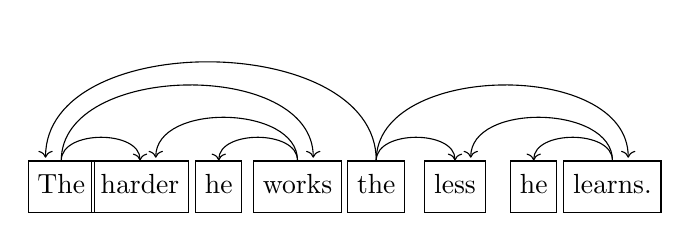
\begin{tikzpicture}[node distance=1cm, on grid=false]%das hilft leider nicht… node spacing ist Kraut&Rüben :'/
\node[draw](the1) at (0,0){\strut The};
\node[draw](harder)[right of=the1]{\strut harder};
\node[draw](he1)[right of=harder]{\strut he};
\node[draw](works)[right of=he1]{\strut works};
\node[draw](the2)[right of=works]{\strut the};
\node[draw](less)[right of=the2]{\strut less};
\node[draw](he2)[right of=less]{\strut he};
\node[draw](learns)[right of=he2]{\strut learns.};
\draw[->] (the1)[out=north,in=north] to (harder);
\draw[->] (the1)[out=north,in=north] to (3.2,.37);
\draw[->] (the2)[out=north,in=north] to (-0.2,.37);
\draw[->] (works)[out=north,in=north] to (he1);
\draw[->] (works)[out=north,in=north] to (1.2,.37);
\draw[->] (the2)[out=north,in=north] to (less);
\draw[->] (the2)[out=north,in=north] to (7.2,.37);
\draw[->] (learns)[out=north,in=north] to (he2);
\draw[->] (learns)[out=north,in=north] to (5.2,.37);
\end{tikzpicture}
	\caption{A WG sketch of the comparative correlative}
	\label{fig:14}
\end{figure}	

Example (\ref{ex:23}) is offered by Jackendoff as a clear case of headlessness, but there is an equally obvious headed analysis of \emph{student after student} in which the structure is the same as in commonplace N P N examples like \emph{box of matches}. The only peculiarity of Jackendoff’s example is the lexical repetition, which is beyond most theories of syntax. For WG, however, the solution is easy: the second N token isa the first, which allows default inheritance. This example illustrates an idiomatic but generalisable version of the N P N pattern in which the second N isa the first and the meaning is special; as expected, the pattern is recursive. The grammatical subnetwork needed to generate the syntactic structure for such examples is shown (with solid lines) in Figure \ref{fig:15}; the semantics is harder and needs more research. What this diagram shows is that there is a subclass of nouns called here “noun\textsubscript{npn}”, which is special in having as its complement a preposition with the special property of having another copy of the same noun\textsubscript{npn} as its complement. The whole construction is potentially recursive because the copy itself inherits the possibility of a preposition complement, but the recursion is limited by the fact that this complement is optional (shown as ‘0,1’ inside the box, meaning that its quantity is either 0 (absent) or 1 (present)). Because the second noun isa the first, if it has a prepositional complement this is also a copy of the first preposition – hence \emph{student after student after student}, whose structure is shown in Figure \ref{fig:15} with dashed lines.

\begin{figure}
	\centering
\begin{tikzpicture}[node distance=1.5cm]
\node[draw](noun) at (0,0){\strut noun};
%first row
\node[draw](nounnpn)[below of=noun, node distance=2.5cm]{\strut noun\textsubscript{npn}};
\node[draw,ellipse](c1)[above right of=nounnpn]{c};
\node[draw](1a)[below right of=c1]{1};
\node[draw](prep)[above of=1a, node distance=2.5cm]{\strut preposition};
\node[draw,ellipse](c2)[above right of=1a]{c};
\node[draw](1b)[below right of=c2]{1};
\node[draw,ellipse](c3)[above right of=1b]{c};
\node[draw](10)[below right of=c3]{1,0};
%second row
\node[draw,dashed](student1)[below of=nounnpn, node distance=2.6cm]{\strut \emph{student}};
\node[draw,ellipse,dashed](c4)[above right of=student1]{c};
\node[draw,dashed](after1)[below right of=c4]{\strut \emph{after}};
\node[draw,ellipse,dashed](c5)[above right of=after1]{c};
\node[draw,dashed](student2)[below right of=c5]{\strut \emph{student}};
\node[draw,ellipse,dashed](c6)[above right of=student2]{c};
\node[draw,dashed](after2)[below right of=c6]{\strut \emph{after}};
\node[draw,ellipse,dashed](c7)[above right of=after2]{c};
\node[draw,dashed](student3)[below right of=c7]{\strut \emph{student}};
%%arrows
\draw[<-,>=open triangle 90 reversed] (noun) to (nounnpn);
\draw[<-,>=open triangle 90 reversed] (prep) to (1a);
\draw[<-,>=open triangle 90 reversed,dashed] (nounnpn) to (student1);
\draw (1b) to[out=south west,in=south east] (0,-3);
%first row
\draw (nounnpn) to (c1);
\draw[->] (c1) to (1a);
\draw (1a) to (c2);
\draw[->] (c2) to (1b);
\draw (1b) to (c3);
\draw[->] (c3) to (10);
%second row
\draw[dashed] (student1) to (c4);
\draw[->,dashed] (c4) to (after1);
\draw[dashed] (after1) to (c5);
\draw[->,dashed] (c5) to (student2);
\draw[dashed] (student2) to (c6);
\draw[->,dashed] (c6) to (after2);
\draw[dashed] (after2) to (c7);
\draw[->,dashed] (c7) to (student3);
\end{tikzpicture}
	\caption{The N P N construction in Word Grammar}
	\label{fig:15}
\end{figure}

The “exhaustive conditional” or “unconditional” in (\ref{ex:24}) clearly has two parts: \emph{however smart} and \emph{the students}, but which is the head? A verb could be added, giving \emph{however smart the students are}, so if we assumed a covert verb that would provide a head, but without a verb it is unclear – and indeed this is precisely the kind of subject-predicate structure that stood in the way of dependency analysis for nearly two thousand years.

However, there are good reasons for rejecting covert verbs in general. For instance, in Arabic a predicate adjective or nominal is in different cases according to whether “be” is overt: accusative when it is overt, nominative when it is covert. Moreover, the word order is different in the two constructions: the verb normally precedes the subject, but the verbless predicate follows it. In Arabic, therefore, a covert verb would simply complicate the analysis; but if an analysis without a covert verb is possible for Arabic, it is also possible in English.

Moreover, even English offers an easy alternative to the covert verb based on the structure where the verb \textsc{be} is overt. It is reasonably uncontroversial to assume a raising analysis for examples such as (\ref{ex:25}) and (\ref{ex:26}), so (\ref{ex:27}) invites a similar analysis \todo{Müller 2013}.

\begin{exe}
	\ex \label{ex:25} He keeps talking.

	\ex \label{ex:26} He is talking.

	\ex \label{ex:27} He is cold.
\end{exe}

But a raising analysis implies a headed structure for \emph{he cold} in which \emph{he} depends (as subject) on \emph{cold}. Given this analysis, the same must be true even where there is no verb, as in example (\ref{ex:24}) \emph{however smart the students} or so-called “Mad-Magazine sentences” like (\ref{ex:28}) \todo{Lambrecht 1990}.%
%
\footnote{A reviewer asks what excludes alternatives such as He smart? and Him smart. (i.e. as a statement. The former is grammatically impossible because he is possible only as the subject of a tensed verb, but presumably the latter is excluded by the pragmatic constraints on the “Mad-magazine” construction.}%
%

\begin{exe}
	\ex \label{ex:28} What, him smart? You’re joking!
\end{exe}

Comfortingly, the facts of exhaustive conditionals support this analysis because the subject is optional, confirming that the predicate is head.

\begin{exe}
	\ex \label{ex:29} However smart, nobody succeeds without a lot of effort.
\end{exe}

In short, where there is just a subject and a predicate, without a verb, then the predicate is the head.

Clearly it is impossible to prove the non-existence of headless phrases, but the examples considered have been offered as plausible examples, so if even they allow a well-motivated headed analysis, it seems reasonable to hypothesise that all phrases have heads.


%%%%%%%%%%%%%%%%%%%%%%%%%%%%%%%%
\subsection{Complex dependency}
\label{sec:5.2}

The differences between HPSG and WG raise another question concerning the geometry of sentence structure because the possibilities offered by the part-whole relations of HPSG are more limited than those offered by the word-word dependencies of WG. How complex can dependencies be? Is there a theoretical limit such that some geometrical patterns can be ruled out as impossible? Two particular questions arise:

\begin{enumerate}
	\item \label{it:4} Can a word depend on more than one other word? This is of course precisely what structure sharing allows, but this only allows “raising” or “lowering” within a single chain of dependencies. Is any other kind of “double dependency” possible?
	
	\item \label{it:5} Is mutual dependency possible?
\end{enumerate}

The answer to both questions is yes for WG, but is less clear for HPSG.

Consider the dependency structure for an example such as (\ref{ex:30}).

\begin{exe}
	\ex \label{ex:30} I wonder who came.
\end{exe}
	
In a dependency analysis the only available units are words, so the clause \emph{who came} has no status in the analysis and is represented by its head. In WG, this is \emph{who} because this is the word that links \emph{came} to the rest of the sentence.

Of interest in (\ref{ex:30}) are three dependencies:

\begin{enumerate}
	\item \label{it:6} \emph{who} depends on \emph{wonder} because \emph{wonder} needs an interrogative complement – i.e. an interrogative word such as \emph{who} or \emph{whether}; so \emph{who} is the object of \emph{wonder}.
	
	\item \label{it:7} \emph{who} also depends on \emph{came} because it is the subject of \emph{came}.
	
	\item \label{it:8} \emph{came} depends on \emph{who}, because interrogative pronouns allow a following finite verb (or, for most but not all pronouns, an infinitive as in \emph{I wonder who to invite}). Since this is both selected by the pronoun and optional (as in \emph{I wonder who}), it must be the pronoun’s complement, so \emph{came} is the complement of \emph{who}.
\end{enumerate}

Given the assumptions of DS, and of WG in particular, each of these dependencies is quite obvious and uncontroversial when considered in isolation. The problem, of course, is that they combine in an unexpectedly complicated way; in fact, this one example illustrates both the complex conditions defined above: \emph{who} depends on two words which are not otherwise syntactically connected (\emph{wonder} and \emph{came}), and \emph{who} and \emph{came} are mutually dependent. A WG analysis of the relevant dependencies is sketched in Figure \ref{fig:16} (where “s” and “c” stand for “subject” and “complement”).

\begin{figure}
	\centering
\begin{tikzpicture}[node distance=1.3cm]
\node[draw](I) at (0,0){\strut ~~I~~ };
\node[draw,ellipse](s1)[above right of=I]{s};
\node[draw](wonder)[below right of=s1]{\strut wonder};
\node[draw,ellipse](c1)[above right of=wonder]{c};
\node[draw](who)[below right of=c1]{\strut who};
\node[draw,ellipse](c2)[above right of=who]{c};
\node[draw](came)[below right of=c2]{\strut came};
\node[draw,ellipse](s2)[above of=c2]{s};
\draw (wonder) to (s1);
\draw[->] (s1) to (I);
\draw (wonder) to (c1);
\draw[->] (c1) to (who);
\draw (who) to (c2);
\draw[->] (c2) to (came);
\draw (came) to (s2);
\draw[->] (s2) to (who);
\end{tikzpicture}
	\caption{Complex dependencies in a relative clause}
	\label{fig:16}
\end{figure}

A similar analysis applies to relative clauses. For instance, in (\ref{ex:31}) the relative pronoun who depends on the antecedent man as an adjunct and on called as its subject, while the ‘relative verb’ called depends on who as its obligatory complement.

\begin{exe}
	\ex \label{ex:31} I knew the man who called.
\end{exe}

Pied-piping presents well-known challenges. Take, for example, (\ref{ex:32}) \citep[212]{ps2}.

\begin{exe}
	\ex \label{ex:32} Here’s the minister [[in [the middle [of [whose sermon]]]] the dog barked]
\end{exe}

According to WG, \emph{whose} (which as a determiner is head of the phrase \emph{whose sermo}n) is both an adjunct of its antecedent \emph{minister} and also the head of the relative verb \emph{barked}, just as in the simpler example. The challenge is to explain the word order: how can \emph{whose} have dependency links to both \emph{minister} and \emph{barked} when it is surrounded, on both sides, by words on which it depends? Normally, this would be impossible, but pied-piping is special. The WG analysis \todo{Hudson 2018} locates the peculiarities of pied-piping entirely in the word order, invoking a special relation ‘pipee’ which transfers the expected positional properties of the relative pronoun (the ‘piper’) up the dependency chain – in this case, to the preposition \emph{in}.

And so we finish this review of complex dependencies by answering the question that exercised the minds of the Arabic grammarians in the Abbasid Caliphate: is mutual dependency possible? The arrow notation of WG allows grammars to generate the relevant structures, so the answer yes, and HPSG can presumably achieve the same effect by means of re-entrance; so this conclusion reflects another example of theoretical convergence.


%%%%%%%%%%%%%%%%%%%%%%%%%%%%%%%%
\subsection{Grammatical functions}
\label{sec:5.3}

As I have already explained, more or less traditional grammatical functions such as subject and adjunct play a central part in WG, and more generally, they are highly compatible with any version of DS because they are all sub-divisions of the basic function dependent. This being so, we can define a taxonomy of functions such as the one in Figure \ref{fig:8} which is developed in Figure \ref{fig:17} to accommodate an example of the very specific functions which are needed in any complete grammar: the second complement of \emph{from}, as in \emph{from London to Edinburgh}, which may be unique to this particular preposition.

\begin{figure}
	\centering
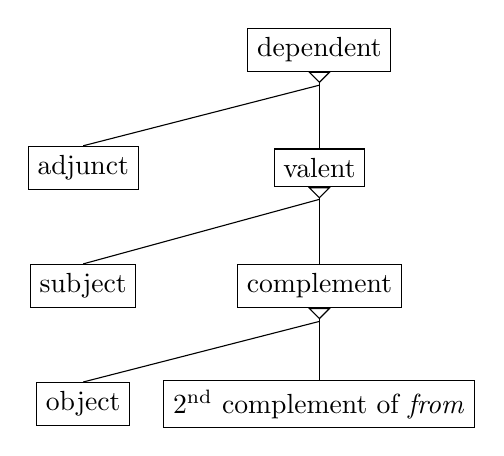
\begin{tikzpicture}[node distance=1.5cm]
%first row
\node[draw](object) at (0,0){object};
\node[draw](comp2)[right of=object, node distance=3cm]{2\textsuperscript{nd} complement of \emph{from}};
%second row
\node[draw](subject)[above of=object]{subject};
\node[draw](comp1)[above of=comp2]{complement};
%third row
\node[draw](adj)[above of=subject]{adjunct};
\node[draw](valent)[above of=comp1]{valent};
%fourth row
\node[draw](dep)[above of=valent]{dependent};
%arrows
\draw[<-,>=open triangle 90 reversed] (dep) to (valent);
\draw[<-,>=open triangle 90 reversed] (valent) to (comp1);
\draw[<-,>=open triangle 90 reversed] (comp1) to (comp2);
%
\draw (object.north) to (3,1.05);
\draw (subject.north) to (3,2.6);
\draw (adj.north) to (3,4.05);
\end{tikzpicture}
	\caption{A taxonomy of grammatical functions}
	\label{fig:17}
\end{figure}

HPSG also recognises a taxonomy of functions by means of three lists attached to any head word.

\begin{description}
	\item[\textnormal{\textsc{spr:}}] \label{it:spr} the word’s specifier, i.e. for a noun its determiner and (in some versions of HPSG) for a verb its subject
	
	\item[\textnormal{\textsc{comps:}}] \label{it:comps} its complements
	
	\item[\textnormal{\textsc{arg-st:}}] \label{it:arg-st} its specifier and its complements, i.e., in WG terms, its valents
\end{description}

The third list concatenates the first two, so the same analysis could be achieved in WG by a taxonomy in which \textsc{spr} and \textsc{comps} both isa \textsc{arg-st}. However, there are also two important differences: in HPSG adjuncts have a different status from other dependents, and these three general categories are lists.

Adjuncts are treated differently in the two theories. In WG, they are dependents, and located in the same taxonomy as valents; so in HPSG terms they would be listed among the head word’s attributes, along with the other dependents but differentiated by not being licensed by the head. But HPSG reverses this relationship by treating the head as a \textsc{mod} (“modified”) of the adjunct. For example, in (\ref{ex:33}) \emph{she} and \emph{it} are listed in the \textsc{arg-st} of \emph{ate} but \emph{quickly} is not mentioned in the AVM of \emph{ate}; instead, \emph{ate} is listed as \textsc{mod} of \emph{quickly}.

\begin{exe}
	\ex \label{ex:33} She ate it quickly.
\end{exe}

This distinction, inherited from Categorial Grammar, correctly reflects the facts of government: \emph{ate} governs \emph{she} and \emph{it}, but not \emph{quickly}. It also reflects one possible analysis of the semantics, in which \emph{she} and \emph{it} provide built-in arguments of the predicate “eat”, while \emph{quickly} provides another predicate “quick”, of which the whole proposition eat(she, it) is the argument. Other semantic analyses are of course possible, including one in which “manner” is an optional argument; but the proposed analysis is consistent with the assumptions of HPSG.

On the other hand, HPSG also recognises a \textsc{head} constituent in every construction, and in the construction which includes \emph{quickly}, the latter is not the head. So what unifies arguments and adjuncts is the fact of not being heads. In contrast, DS theories (including WG) agree in recognising adjuncts as dependents, so arguments and adjuncts are unified by this category, which is missing from most versions of HPSG, though not from all \citep{BMS2001a}. The DS analysis follows from the assumption that dependency isn’t just about government, nor is it tied to a logical analysis based on predicates and arguments. At least in WG, the basic characteristic of a dependent is that it modifies the meaning of the head word, so that the resultant meaning is (typically) a hyponym of the head’s unmodified meaning. Given this characterisation, adjuncts are core dependents; for instance \emph{big book} is a hyponym of \emph{book} (i.e. “big book” isa “book”), and \emph{she ate it quickly} is a hyponym of \emph{she ate it}. The same characterisation also applies to arguments: \emph{ate it} is a hyponym of \emph{ate}, and \emph{she ate it} is a hyponym of \emph{ate it}. (Admittedly hyponymy is merely the default, and as explained in section \ref{sec:4.1} it may be overridden by the details of particular adjuncts such as \emph{fake} as in \emph{fake diamonds}; but exceptions are to be expected.)

Does the absence in HPSG of a unifying category “dependent” matter? So long as \textsc{head} is available, we can express word-order generalisations for head-final and head-initial languages, and maybe also for “head-medial” languages such as English \citep[172]{Hudson2010b-u}. At least in these languages, adjuncts and arguments follow the same word-order rules, but although it is convenient to have a single cover term dependent for them it is probably not essential. So maybe the presence of \textsc{head} removes the need for its complement, \textsc{dependent}.

The other difference between HPSG and WG lies in the way in which the finer distinctions among complements are made. In HPSG they are shown by the ordering of elements in a list, whereas WG distinguishes them as further subcategories in a taxonomy. For example, in HPSG the direct object is identified as the second NP in the \textsc{arg-st} list, but in WG it is a sub-category of “complement” in the taxonomy of Figure \ref{fig:17}. In this case, each approach seems to offer something which is missing from the other.

On the one hand, the ordered lists of HPSG reflect the attractive ranking of dependents offered by Relational Grammar \citep{PP83a-u}\todo{PP83a-u hat kein year!!! Blake 1990} in which arguments are numbered from 1 to 3 and can be “promoted” or “demoted” on this scale. The scale had subjects at the top and remote adjuncts at the bottom, and appeared to explain a host of facts from the existence of argument-changing alternations such as passivization \citep{Levin93a-u} to the relative accessibility of different dependents to relativisation \citep{KC77a}. An ordered list, as in \textsc{arg-st}, looks like a natural way to present this ranking of dependents.

On the other hand, the taxonomy of WG functions has the attraction of open-endedness and flexibility, in contrast with the HPSG analysis which assumes a fixed and universal list of dependency types defined by the order of elements in the various categories discussed previously (\textsc{spr}, \textsc{comps} and \textsc{arg-st}). A universal list of categories requires an explanation: Why a universal list? Why this particular list? How does the list develop in a learner’s mind? In contrast, a taxonomy can be learned entirely from experience, can vary across languages, and can accommodate any amount of minor variation. Of these three attractions, the easiest to illustrate briefly is the third. Take once again the English preposition \emph{from}, as in (\ref{ex:34}).

\begin{exe}
	\ex \label{ex:34} From London to Edinburgh is four hundred miles.
\end{exe}

Here \emph{from} seems to have two complements: \emph{London} and to \emph{Edinburgh}. Since they have different properties, they must be distinguished, but how? The easiest and arguably correct solution is to create a special dependency type just for the second complement of \emph{from}. This is clearly unproblematic in the flexible WG approach, where any number of special dependency types can be added at the foot of the taxonomy, but much harder if every complement must fit into a universal list. (Note that the availability of a dustbin category such as “oblique” would not help, because the second complement of \emph{from} has specific syntactic and semantic properties which need to be specified. If a category could be described as a dustbin, it is not a category because it does no work in the inheritance system.)

To summarise the discussion, therefore, HPSG and WG offer fundamentally different treatments of grammatical functions with two particularly salient differences. In the treatment of adjuncts, there are reasons for preferring the WG approach in which adjuncts and arguments are grouped together explicitly as dependents. But in distinguishing different types of complement, the HPSG lists seem to complement the taxonomy of WG, each approach offering different benefits. This is clearly an area needing further research.


%%%%%%%%%%%%%%%%%%%%%%%%%%%%%%%%%%%%%%%%%%%%%%%%%%%%%
%%%%%%%%%%%%%%%%%%%%%%%%%%%%%%%%%%%%%%%%%%%%%%%%%%%%%
\section{HPSG without PS?}
\label{sec:6}

This chapter on HPSG and DS raises a fundamental question for HPSG: does it really need PS? Most introductory textbooks present PS as an obvious and established approach to syntax, but it is only obvious because these books ignore the DS alternative: the relative pros and cons of the two approaches are rarely assessed. Even if PS is in fact better than DS, this can’t be described as “established” (in the words of one of my reviewers) until its superiority has been demonstrated. This hasn’t yet happened. The historical sketch showed very clearly that nearly two thousand years of syntactic theory assumed DS, not PS, with one exception: the subject-predicate analysis of the proposition (later taken to be the sentence). Even when PS was invented by Bloomfield, it was combined with elements of DS, and Chomsky’s PS, purified of all DS elements, only survived from 1957 to 1970.

A reviewer also argues that HPSG is vindicated by the many large-scale grammars that use it. These grammars are indeed impressive, but DS theories have also been implemented in the equally large-scale projects listed in Section \ref{sec:2}. In any case, the question is not whether HPSG is a good theory, but rather whether it might be even better without its PS assumptions. The challenge for HPSG, then, is to explain why PS is a better basis than DS. The debate has hardly started, so its outcome is unpredictable; but suppose the debate favoured DS. Would that be the end of HPSG? Far from it. It could survive almost intact, with just two major changes.

The first would be in the treatment of grammatical functions. It would be easy to bring all dependents together in a list called \textsc{deps} \citep{BMS2001a} with \textsc{adjuncts} and \textsc{comps} as sub-lists, or even with a separate subcategory for each sub-type of dependent \todo{Hellan 2017}.

The other change would be the replacement of phrasal boxes by a single list of words. \ref{ex:35} gives a list for the example with which we started (with round and curly brackets for ordered and unordered sets, and a number of sub-tokens for each word):

\begin{exe}
	\ex \label{ex:35} ({\emph{many}, \emph{many}+\emph{h}} {\emph{students}, \emph{students}+\emph{a}}, {\emph{enjoy}, \emph{enjoy}+\emph{o}, \emph{enjoy}+\emph{s}}, \emph{syntax})
\end{exe}

Each word in this list stands for a whole box of attributes which include syntactic dependency links to other words in the list. The internal structure of the boxes would otherwise look very much like standard HPSG, as in the schematic neo-HPSG structure in Figure \ref{fig:18}. (To improve readability by minimizing crossing lines, attributes and their values are separated as usual by a colon, but may appear in either order.)

\begin{figure}
	\centering
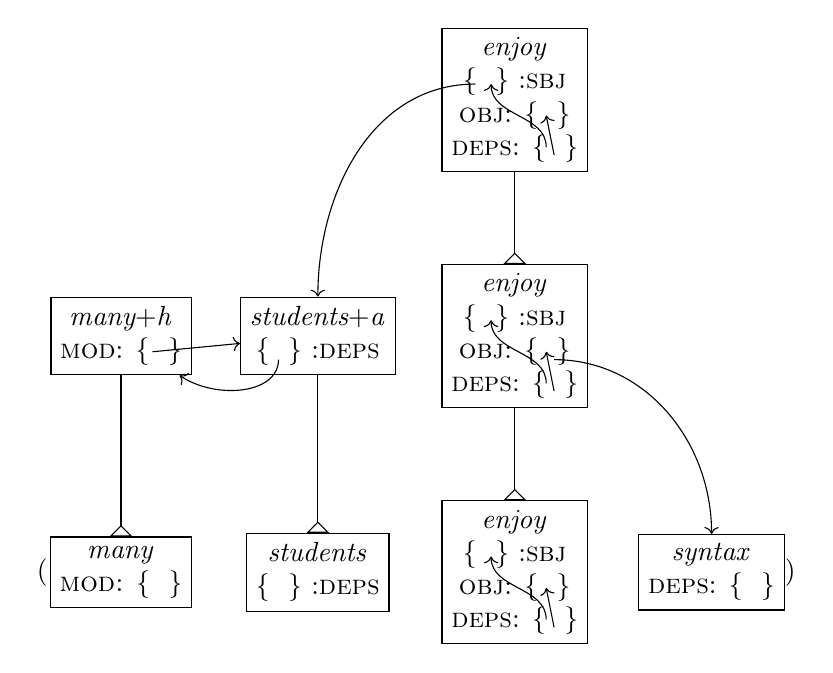
\begin{tikzpicture}[node distance=2.5cm]
%first row
\node[draw, align=center](many1) at (0,0){\emph{many}\\\textsc{mod:} \{~~\}};
\node[draw, align=center](students1)[right of=many1]{\emph{students}\\\{~~\} :\textsc{deps}};
\node[draw, align=center](enjoy1)[right of=students1]{\emph{enjoy}\\\{~~\} :\textsc{sbj}\\\textsc{obj}: \{~~\}\\\textsc{deps}: \{~~\}};
\node[draw, align=center](syntax)[right of=enjoy1]{\emph{syntax}\\\textsc{deps}: \{~~\}};
%second row
\node[draw, align=center](many2)[above of=many1, node distance=3cm]{\emph{many$+$h}\\\textsc{mod}: \{~~\}};
\node[draw, align=center](students2)[right of=many2]{\emph{students$+$a}\\\{~~\} :\textsc{deps}};
\node[draw, align=center](enjoy2)[right of=students2]{\emph{enjoy}\\\{~~\} :\textsc{sbj}\\\textsc{obj}: \{~~\}\\\textsc{deps}: \{~~\}};
%third row
\node[draw, align=center](enjoy3)[above of=enjoy2, node distance=3cm]{\emph{enjoy}\\\{~~\} :\textsc{sbj}\\\textsc{obj}: \{~~\}\\\textsc{deps}: \{~~\}};
%arrows
\draw[<-,>=open triangle 90 reversed] (many1) to (many2);
\draw[<-,>=open triangle 90 reversed] (students1) to (students2);
\draw[<-,>=open triangle 90 reversed] (enjoy1) to (enjoy2);
\draw[<-,>=open triangle 90 reversed] (enjoy2) to (enjoy3);
%%%
\draw[->] (.4,2.8) to (students2);
\draw[->] (2,2.7) to[in=south east, out=south] (many2);
\draw[->] (4.5,6.2) to[in=north, out=west] (students2);
\draw[->] (5.5,2.7) to[in=north, out=east] (syntax);
%%%
\draw[->] (5.5,-.7) to (5.4,-.2);
\draw[->] (5.4,-.6) to[in=south, out=north] (4.7,.2);
%
\draw[->] (5.5,2.3) to (5.4,2.8);
\draw[->] (5.4,2.4) to[in=south, out=north] (4.7,3.2);
%
\draw[->] (5.5,5.3) to (5.4,5.8);
\draw[->] (5.4,5.4) to[in=south, out=north] (4.7,6.2);
%braces
\node(b1)[left of=many1, node distance=1cm]{(};
\node(b2) [right of=syntax, node distance=1cm]{)};
\end{tikzpicture}
	\caption{A neo-HPSG analysis}
	\label{fig:18}
\end{figure}

Figure \ref{fig:18} can be read as follows:

\begin{itemize}
	\item The items at the bottom of the structure (\emph{many}, \emph{students}, \emph{enjoy} and \emph{syntax}) are basic types stored in the grammar, available for modification by the dependencies. These four words are the basis for the ordered set in (\ref{ex:35}), and shown here by the round brackets, with the ordering shown by the left-right dimension. This list replaces the ordered partonomy of HPSG.

	\item Higher items in the vertical taxonomy are tokens and sub-tokens, whose names show the dependency that defines them (\emph{h} for “head”, \emph{a} for “adjunct”, and so on). The taxonomy above \emph{enjoy} shows that \emph{enjoy}+\emph{s} isa \emph{enjoy}+\emph{o} which isa \emph{enjoy}, just as in an HPSG structure where each dependent creates a new representation of the head by satisfying and cancelling a valency need and passing the remaining needs up to the new representation.

	\item The taxonomy above \emph{students} shows that \emph{students}+\emph{a} is a version of \emph{students} that results from modification by \emph{many}, while the parallel one above \emph{many} shows that (following HPSG practice) \emph{many}+\emph{h} has the function of modifying \emph{students}.
\end{itemize}

Roughly speaking, each boxed item in this diagram corresponds to an AVM in a standard HPSG analysis.

In short, modern HPSG could easily be transformed into a version of DS, with a separate AVM for each word. As in DS, the words in a sentence would be represented as an ordered list interrelated partly by the ordering and partly by the pairwise dependencies between them. This transformation is undeniably possible. Whether it is desirable remains to be established by a programme of research and debate which will leave the theory more robust and immune to challenge.


\section*{Abbreviations}
\section*{Acknowledgements}

%\bibliography{../Bibliographies/stmue}
\printbibliography[heading=subbibliography,notkeyword=this] 
\end{document}
